\documentclass[12pt,twoside,openright]{report}
\usepackage{minted}
\usepackage{xcolor}
\definecolor{light-gray}{rgb}{0.9,0.9,0.9}
\usepackage{emptypage}
\usepackage[T1]{fontenc}
\usepackage{textcomp}
\usepackage[utf8]{inputenc}
\usepackage[italian]{babel}
\usepackage{graphicx}
\graphicspath{ {immagini/} }
\usepackage{caption}
\usepackage{subcaption}
\usepackage[a4paper,width=150mm,top=30mm,bottom=30mm,left=30mm,right=30mm,bindingoffset=6mm]{geometry}
\usepackage{fancyhdr}
\pagestyle{fancy}
\setlength{\headheight}{15pt}% 
\fancyhead{}
\fancyhead[LE, RO]{\leftmark}
\fancyfoot{}
\fancyfoot[LE,RO]{\thepage}
\renewcommand{\headrulewidth}{0.4pt}
\renewcommand{\footrulewidth}{0.4pt}
\linespread{1.5}\selectfont

\begin{document}

  \shipout\null  

  \thispagestyle{plain}
\chapter*{Abstract}

Il continuo sviluppo delle tecnologie di apprendimento automatico ha reso più semplice ed efficace il monitoraggio dei dati relativi alla salute dell’uomo. L’obiettivo di questa tesi è quello di estrarre ed elaborare informazioni a partire da immagini dell’iride al fine di poterle utilizzare come strumento diagnostico. Il software è composto da due parti, la prima legata all’elaborazione dell’immagine, in particolare applicazione di filtri adeguati e metodi di riconoscimento, segmentazione e scaling dell’iride. La seconda parte rielabora i dati ricavati precedentemente al fine di poterli utilizzare in opportuni algoritmi di machine learning. L'implementazione proposta utilizza come strumento di apprendimento automatico una Convolutional Neural Network (CNN) per studiare la veridicità dell’iridologia, una tecnica alternativa di diagnosi che si basa sull’analisi di sezioni dell’iride.

  
  \tableofcontents
  
  \chapter{Introduzione}
  Negli ultimi anni l’analisi dell’occhio si è rivelata particolarmente interessante in diversi ambiti, quali sicurezza, scanner biometrici, identificazione di persone, medicina, etc. In particolar modo l’iride è la porzione dell’occhio che contiene la maggior parte delle informazioni utili a fini scientifici. 

In questo progetto di tesi si esplorano le diverse tecniche di elaborazione di immagini dell’occhio al fine di individuare ed estrapolare regioni di interesse dell’iride (settori di iride chiamati ROI). Lo scopo finale è quello di utilizzare queste regioni come dato fondamentale per effettuare analisi di vario tipo con un approccio alternativo; tuttavia di per sé le zone d’interesse trovate non risultano sufficienti a tale scopo, è necessario dunque inserire un ulteriore metodo che analizzi queste regioni in modo tale da produrre una valutazione il più possibile accurata. Come metodo di valutazione si è pensato di cercare uno strumento che fosse in grado di riconoscere i pattern comuni all’interno dei segmenti precedentemente individuati. La scelta è immediatamente ricaduta su una branca dell’intelligenza artificiale in rapido sviluppo, il machine learning. Esistono infatti opportuni modelli particolarmente adatti a questo problema. Tali modelli saranno approfonditi in seguito in questa trattazione, illustrandone le potenzialità e il funzionamento. L’impiego combinato di tecnologie di apprendimento automatico e di analisi/elaborazione delle immagini risulta quindi efficace per la creazione di modelli che producano, partendo da semplici immagini dell’occhio, una analisi accurata in modo automatico. 

Il caso d’uso preso in considerazione per lo studio e l’applicazione dei metodi di elaborazione di immagini e degli algoritmi di machine learning è quello dell’iridologia, una teoria medica non ancora validata. L’obiettivo finale vuole essere quello di confrontare i risultati ottenuti da un modello adeguatamente accurato, creato sulla base delle immagini dell’iride, con quelli sostenuti dell'iridologia al fine di confermare la veridicità o meno della suddetta teoria. 

 

  
  
  \chapter{}
  \section{Nozioni di iridologia}
  L’iridologia è una pratica pseudoscientifica di diagnosi basata sull’osservazione dell’iride.  È considerata una medicina alternativa in quanto non esiste alcun riscontro medico/scientifico che convalidi le sue teorie.  Secondo l’iridologia, l’iride è divisa in specifiche sezioni che corrispondono a specifiche parti del corpo. Le immagini seguenti rappresentano la mappa delle zone d’interesse creata dal Dr. Bernard Jensen, uno dei pionieri della teoria.

\begin{figure}[h]
  \centering
  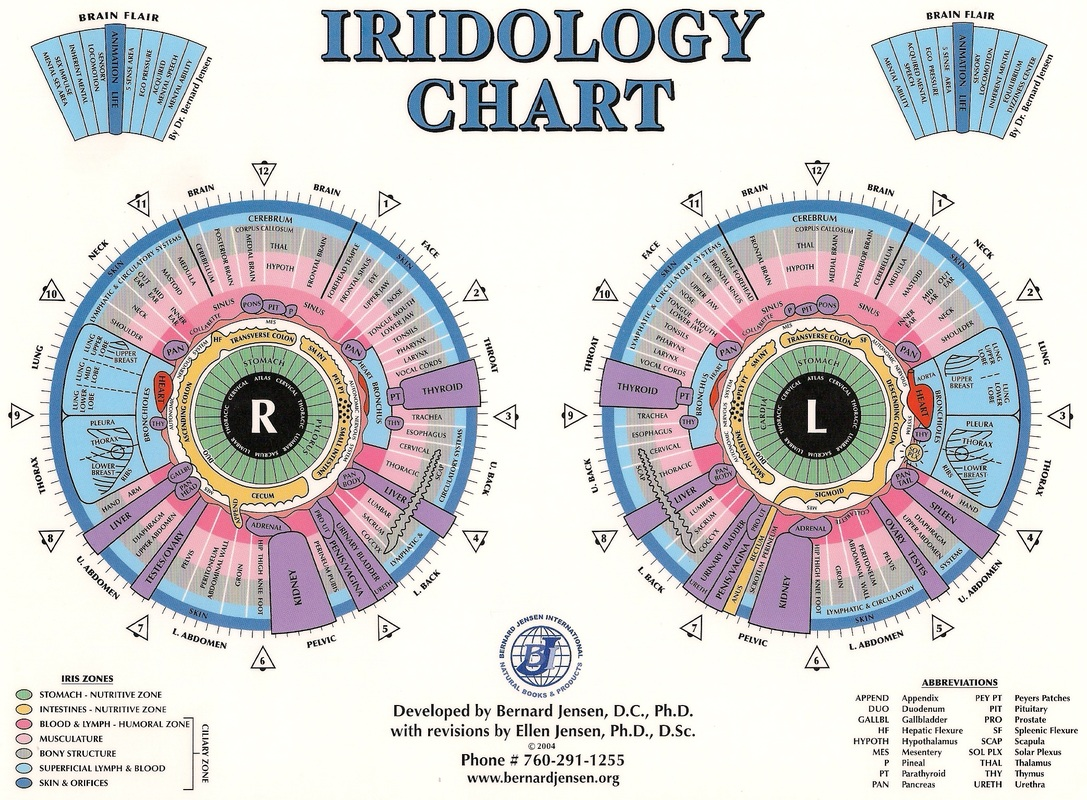
\includegraphics[scale=0.7]{iridology_chart}
  \caption{Mappa dell'iride del Dr. Bernard Jensen}
\end{figure}

Nella mappa sono state individuate 166 aree di cui 80 nell’iride destra e 86 in quella sinistra. Gli iridologi sostengono che guardando una particolare sezione dell’iride, in accordo alla mappa sopracitata, si può determinare, anche in assenza di sintomi, l’esistenza o meno di un problema nella regione del corpo relativa al segmento in esame; tuttavia la teoria non definisce quale sia la presunta malattia. Nella pratica gli iridologi generalmente usano strumenti come microscopi o lenti di ingrandimento per verificare cambiamenti nell’iride, in particolare si cercano specifici pattern di colori o irregolarità nel tessuto dell’occhio. I risultati sono poi comparati con la mappa per correlare le zone affette ai relativi organi. Quindi tutto ciò significa che un’eventuale malattia si dovrebbe riflettere in un evidente cambiamento in qualche sezione dell’iride. Molti studi tuttavia hanno dimostrato che non c’è diretta correlazione tra malattia e iride ed è per questo che la maggior parte dei dottori rigetta questa teoria. 
  
  \section{Algoritmi di apprendimento automatico applicati all'iridologia}
  Nel seguente progetto si è cercato di utilizzare un approccio alternativo alle classiche ricerche mediche per dare un parere relativo alla veridicità o meno dell’iridologia. Si è pensato di utilizzare il Machine Learning: esso è lo studio scientifico di algoritmi che creano modelli matematico-statistici, basati sull’inferenza e la ricerca di pattern nei dati, affinché una macchina possa effettuare previsioni senza che venga esplicitamente programmata per farlo. L’accuratezza di tali previsioni è legata al processo di ricerca dei pattern sopracitato, detto anche processo di training: il modello apprenderà le variazioni tra questi dati di training e le utilizzerà per capire quale previsione dare in output a fronte di un nuovo dato. La precisione di queste previsioni sarà quindi strettamente legata ai dati su cui si fa training del modello in riferimento alla quantità e qualità di essi. L’approccio alternativo si basa sull’utilizzo di un modello, opportunamente accurato, che sia in grado, partendo da un segmento di iride legato ad una parte del corpo secondo la mappa dell’iridologia, di produrre in output una predizione riguardo la presenza o meno di un problema relativo alla parte del corpo associata al suddetto segmento. In questo modo si può confrontare il risultato prodotto dal modello con il parere di un iridologo; se nella maggior parte dei casi i pareri risultano discordanti significa che, con buona probabilità, non c’è una correlazione diretta tra iride e patologia. 

Tuttavia è doveroso fare alcune premesse: il modello utilizzato, al fine di produrre previsioni il più possibile corrette, deve avere una buona accuratezza; inoltre, per garantire la validità delle previsioni, è necessario fare training su immagini che abbiano una vera validità medica. Ad esempio: se si vuole cercare il riscontro di un problema al cuore sull’iride, bisogna fare training con segmenti relativi alla sezione dell’iride dedicata al cuore sia di persone di cui si conosce per certo l’esistenza di un problema al cuore sia di persone che non hanno nessun problema all’organo. In questo modo il modello imparerà a capire se vi è una relazione tra porzione di iride e problema al cuore. Una predizione prodotta dal modello ed una valutazione fatta da un iridologo possono poi essere confrontata con il parere di un medico professionista per avere un riscontro oggettivo. Per poter ottenere questo obiettivo si è ricercato un modello che fosse in grado di analizzare immagini al fine di capirne i pattern. Il modello più idoneo per questo tipo di problema è quello delle Convolutional Neural Network (CNN), una sottoclasse di modelli di machine learning dette Artificial Neural Network. Una descrizione più dettagliata delle CNN verrà trattata nel capitolo 6.2.


  
  \chapter{Struttura del progetto}
  \section{Tecnologie}
  Per la realizzazione dell’intero progetto si è utilizzato come linguaggio di programmazione Python 3. Si è scelto questo linguaggio per diversi motivi, il primo in assoluto è relativo al fatto che python rappresenta il linguaggio maggiormente utilizzato nello sviluppo di applicazioni legate al mondo del Machine Learning, difatti i più moderni framework per l’apprendimento automatico, come Tensorflow ad esempio, sono sviluppati in python. Tuttavia, questo non è l’unico motivo, anzi, ci sono altre ragioni che hanno portato alla scelta di questo linguaggio, ad esempio altri punti di forza di python sono la semplicità, la flessibilità e la versatilità, è infatti disponibile sulle principali piattaforme in circolazione (Windows, Linux e Mac OS). Altre caratteristiche sono il supporto di più paradigmi, tra cui: object oriented, strutturale e funzionale e la grande disponibilità di moduli pronti all’uso che permettono di arricchire il set di funzioni base del linguaggio. 
Tra i diversi moduli utilizzati nell’applicativo i principali sono:
\begin{itemize}
  \item \textbf{Python - OpenCV (cv2)}:  OpenCV sta per Open Source Computer Vision Library; Python - OpenCV è la versione python della popolare libreria utilizzata per la visione artificiale. Nel progetto viene utilizzata per le varie funzioni di elaborazione delle immagini
  \item \textbf{Numpy}: questa libreria aggiunge al linguaggio il supporto di array multidimensionali e matrici anche di grandi dimensioni; inoltre aggiunge anche molte funzioni matematiche di altro livello utili per operare con questo tipo di dati
  \item \textbf{Tensorflow}: framework sviluppato per l’apprendimento automatico. Contiene una vasta gamma di funzionalità legate al mondo del Machine Learning, fornisce moduli ottimizzati per la realizzazione di algoritmi o modelli di ML. Nell’ applicativo viene utilizzato soprattutto per la creazione della rete neurale
  \item \textbf{ConfigParser}: libreria che implementa un file parser per gestire file di configurazione strutturati
  \item \textbf{os}: modulo nativo di python che permette di utilizzare funzioni del sistema operativo. Ad esempio nel progetto viene spesso utilizzato per fare controlli su file, creare/eliminare cartelle e gestire path
\end{itemize}


  \section{Struttura del codice}
  Il progetto è composto da una serie di script python; la maggior parte è organizzata in moduli, ovvero collezioni di script che contengono solo funzioni o costanti, oltre a questi file sono anche presenti tre script direttamente eseguibili che richiamano le funzioni offerte da tali moduli.

I due moduli creati sono:
\begin{itemize}
  \item \textbf{Preprocessing}: contiene gli script necessari alla fase preparazione dei dati per il training della rete neurale. In particolare contiene tutte le funzioni per l’elaborazione delle immagini, come filtri, metodi di riconoscimento dell’iride, etc...
  \item \textbf{ML\_CNN}:  contiene gli script che permettono di creare, fare training e deploy del modello di rete neurale  
\end{itemize}

Gli script principali, ovvero quelli che poi verranno effettivamente mandati in esecuzione,  sono tre: \texttt{preprocess.py}, \texttt{train.py} e \texttt{predict.py}. \texttt{Preprocess.py} richiama le funzioni offerte dal modulo Preprocessing per elaborare le immagini in input al fine di  creare in output le immagini del segmento di iride selezionato. Lo script \texttt{train.py} utilizza le funzioni offerte dal modulo ML\_CNN per creare il dataset di training partendo dai segmenti precedentemente generati; successivamente, richiama i metodi per la generazione e il training del modello, producendo infine in output un file con estensione \texttt{.model} che rappresenta il modello appena creato. Infine lo script \texttt{predict.py} riutilizza il modulo Preprocessing per elaborare le nuove immagini su cui si vuole fare una previsione, così da produrre a sua volta i segmenti di iride. Si usa infine il modello scelto dall’utente e si producono in output le previsioni  generate dalla rete neurale.

  \section{File di configurazione}
  Dato che le diverse funzioni nel codice contengono svariati parametri di configurazione si è pensato di creare un apposito file contenente le associazioni parametro-valore, chiamato \texttt{config.ini}. Il file è strutturato in sezioni ed ogni sezione ha associato un insieme di parametri ad essa relativi; questi rappresentano i parametri fondamentali di tutte le principali funzioni presenti nel programma. Lo scopo di questo file è creare un metodo più rapido e semplice per la modifica dei valori dei parametri, in questo modo un utente che vuole effettuare test diversi, non necessariamente riguardanti l’iridologia, può semplicemente andare a modificare i valori dei parametri di interesse senza dover modificarli direttamente nelle chiamate alle funzioni nel codice.

    
  \chapter{Processi di funzionamento del software e suo utilizzo}
  \section{Premesse}
  E’ necessario fare una serie di premesse riguardo la scelta delle immagini da utilizzare nel programma, la quale risulta fondamentale per il corretto funzionamento dello stesso. Le immagini che verranno processate e successivamente utilizzate nel modello di training devono avere la stessa dimensione (non troppo piccola), in quanto dimensioni differenti porterebbero ad avere errori nel riconoscimento dell’iride e della pupilla. Le foto dell’occhio devono essere scattate frontalmente, poiché il programma non è sempre in grado di riconoscere l’iride se l’occhio è trasversale. E’ inoltre molto importante che l’occhio sia ben aperto, limitando il più possibile la presenza delle palpebre, in quanto risulterebbe falsata l’analisi di un segmento che le contiene anche solo parzialmente. 

\begin{figure}
  \centering
  \begin{subfigure}[b]{0.4\textwidth}
    \centering
    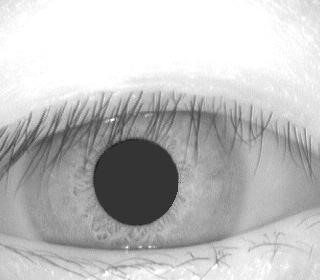
\includegraphics[width=\textwidth]{premesse_1}
    \caption{Immagine non ottimale}    
  \end{subfigure}
  \hfill
  \begin{subfigure}[b]{0.4\textwidth}
    \centering
    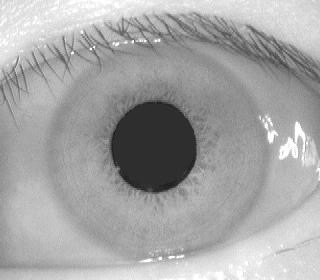
\includegraphics[width=\textwidth]{premesse_2}
    \caption{Immagine ottimale}       
  \end{subfigure}
  \caption{Esempi di immagini presenti nel dataset CASIA}
\end{figure}

Inoltre affinché un modello di machine learning produca risultati attendibili nel caso d’uso trattato, si dovrebbe utilizzare idealmente un elevato numero di immagini, equamente distribuite nelle classi di training. Un’ultima, importante premessa, va fatta riguardo il file di configurazione. In esso i parametri  sono settati appositamente per l’implementazione proposta. L’utilizzo di immagini differenti, in particolar modo di dimensioni diverse da quelle del dataset utilizzato in questo lavoro, comporta una dovuta modifica di alcuni di questi parametri, a carico dell’utente. Se non vengono modificati correttamente, i risultati dell’elaborazione potrebbero portare allo scarto di numerose immagini in seguito, ad esempio,  alla non corretta identificazione dei segmenti. 

  \section{Panoramica del flusso d'esecuzione}
  Di seguito verrà fatta una descrizione generalizzata del processo di funzionamento del software, mentre nei capitoli successivi si andranno a descrivere più nel dettaglio le singole parti del codice che portano all’obiettivo finale. Il codice è suddiviso in tre macro-sezioni: la sezione di elaborazione delle immagini, la sezione dedicata al machine learning e infine la sezione che si occupa di effettuare le previsioni. Come prima cosa, l’utente inserisce le immagini su cui fare training nella cartella \texttt{DATA\_IMAGES}, in particolare suddivide le immagini in due subset: il set di immagini associate ad un problema andranno inserite nella sottocartella \texttt{DB\_PROBS} mentre il set di immagini che si possono definire senza problematiche va inserito nella sottocartella \texttt{DB\_NORMAL}. Una volta inseriti i dati si può procedere all’esecuzione dello script \texttt{preprocess.py}: tale script, come già anticipato, carica le immagini collocate nella cartella \texttt{DATA\_IMAGES} e successivamente richiama diverse funzioni di elaborazione delle immagini. Le immagini processate vengono poi inviate alle funzioni di riconoscimento di iride e pupilla, quelle con un riscontro positivo passano poi alla funzione di segmentazione e crop, infine si procede al resize dei segmenti ad una dimensione fissa e al salvataggio. Alla fine di questo sottoprocesso lo script crea nella cartella root del progetto una sottocartella chiamata \texttt{TEMP\_SEG}, contenente a sua volta due sottocartelle chiamate \texttt{DB\_NORMAL\_SEG} e \texttt{DB\_PROBS\_SEG}. All’interno di esse troviamo rispettivamente i segmenti di iride elaborati relativi  alle immagini in \texttt{DB\_NORMAL} e in \texttt{DB\_PROBS}. E’ importante notare che nel caso di errori durante la fase di “filtraggio” delle immagini oppure nel caso di errori dovuti alla mancata rilevazione o rilevazione errata dell’iride/pupilla (intesa come rilevazione di più di un’iride/pupilla)  il programma provvede a scartare l’immagine; quindi il numero segmenti in output potrebbe risultare inferiore di quello delle immagini in input. Una volta generati i segmenti si procede con il training della rete neurale. Per far ciò si manda in esecuzione lo script \texttt{train.py}, che carica le immagini dei segmenti e li organizza in una struttura dati che può essere analizzata dalla rete. Una volta ottenuta tale struttura si può passare alla creazione del modello e al training vero e proprio, al termine di tale processo lo script produce in output il file \texttt{.model} che contiene tutte le informazioni relative al modello appena generato. Il modello può essere poi utilizzato nella fase finale, ovvero nella fase di prediction, per fare previsioni. L’utente andrà ad inserire nella cartella \texttt{DATA\_TO\_PREDICT}, sottocartella di \texttt{PREDICTION}, le immagini di cui vuole una previsione, poi inserisce nella cartella \texttt{PREDICTION} il file \texttt{.model} relativo al modello di rete neurale che si vuole utilizzare per fare la previsione. Fatta questa preparazione si esegue lo script \texttt{predict.py} che fa passare le immagini presenti nella cartella \texttt{DATA\_TO\_PREDICT} attraverso le fasi di preprocessing in modo da produrre dei segmenti utilizzabili dal modello preso in esame (in sostanza produce dei segmenti della stessa dimensione dei segmenti usati per fare il training del modello). Infine lo script carica in memoria il modello e chiede alla rete di fare previsioni sui segmenti precedentemente creati, in output l’utente si ritroverà la label (problema o normale) che la rete ha ritenuto opportuno associare a quel segmento. La descrizione appena fatta rappresenta un utilizzo tipico del programma, tuttavia è importante menzionare il fatto che non è obbligatorio fare un’esecuzione sequenziale delle tre macro-sezioni; infatti è possibile per esempio eseguire \texttt{predict.py} su modelli diversi e non necessariamente sull’ultimo modello creato. Di seguito si andrà a fare un descrizione dettagliata delle diverse fasi del processo, relative allo specifico caso d’uso dell’iridologia,  che partendo dalle immagini di input portano alle predizioni finali. E’ doveroso far notare che per poter procedere nella realizzazione dell’elaborato, non avendo a disposizione immagini strettamente legate all’iridologia, si è scelto di utilizzare il dataset CASIA v.4.0, il quale è composto quasi interamente da immagini che soddisfano tutte le premesse fatte in precedenza ma che tuttavia contiene solo immagini di occhi normali (a cui non è associato nessun problema) e quindi non rappresenta un valido dataset per verificare la validità dell’iridologia. Di conseguenza i risultati di training non saranno accurati, ma per l’elaborazione delle immagini ed estrazione dei segmenti il dataset scelto si è rivelato ottimale. Per questo motivo è doveroso dire che il programma non è stato pensato e scritto solo per il caso d’uso dell’iridologia, ma è potenzialmente utilizzabile per ulteriori progetti relativi all’analisi dell’occhio, infatti si presuppone che con le adeguate immagini, categorizzate in modo opportuno, si riescano ad ottenere dei buoni risultati. Detto ciò, le immagini presenti in questo dataset (in seguito alla cancellazione di alcune immagini non soddisfacenti le premesse) sono 488. Si farà spesso riferimento a parametri scelti appositamente per questo caso d’uso, tarati in base alle immagini a disposizione.

  
  \chapter{Elaborazione delle immagini}
  All’avvio dello script \texttt{preprocess.py} viene inocata la funzione \texttt{create\_data} che si occupa di estrarre i segmenti dalle immagini in input, tale risultato è ottenuto invocando una serie di altre funzioni in sequenza che verranno descritte di seguito.

  \section{Caricamento delle immagini}
  La prima funzione è \texttt{load\_image}, si occupa di caricare le immagini presenti nel path passato come parametro e le restituisce come un array di immagini (matrici di pixel). Il path è preimpostato e punta alla cartella \texttt{DATA\_IMAGES} che , come già accennato in precedenza, contiene il dataset di immagini CASIA divise per tipologia. Il caricamento viene reso possibile dalla funzione \texttt{cv2.imread} della libreria OpenCV che carica le immagini come matrici di pixel codificate nel formato BGR (Blue Green Red). Qualora fosse necessario è possibile abilitare a \texttt{True} il parametro \texttt{RESIZE} presente nella sezione \texttt{PREPROCESSING} del file di configurazione,in questo modo viene effettuato un resize automatico sulla base della dimensioni specificate dal parametro \texttt{RESIZE\_SHAPE}, nel nostro caso non è stato necessario fare un resize in quanto tutte le immagini erano già della stessa dimensione (320 x  280). La funzione ritorna l’array di matrici a tre livelli contenenti i valori BGR dei pixel delle immagini e l’array contenente i nomi dei file delle immagini.

  \section{Filtri}
  All’avvio dello script \texttt{preprocess.py} viene inocata la funzione \texttt{create\_data} che si occupa di estrarre i segmenti dalle immagini in input, tale risultato è ottenuto invocando una serie di altre funzioni in sequenza che verranno descritte di seguito.

  \subsection{Trasformazioni morfologiche}
  Una trasformazione morfologica è una semplice operazione  basata sulla shape (high x width) dell’immagine.


\begin{minted}
[
  xleftmargin=\parindent,
  framesep=2mm,
  baselinestretch=1.2,  
  fontsize=\footnotesize,
  linenos
]
{python}

kernel = cv2.getStructuringElement(cv2.MORPH_ELLIPSE, (5, 5))
blackhat = cv2.morphologyEx(cimg, cv2.MORPH_BLACKHAT, kernel)
bottom_hat_filtered = cv2.add(blackhat, cimg)    
\end{minted}

Nel codice sopra riportato la funzione che opera le trasformazioni morfologiche è \texttt{cv2.morphologyEx}, la quale utilizza erosione e dilatazione come operazioni di base. L’erosione consiste nell’erodere i bordi di una forma, un pixel nell’immagine originale in bianco e nero (0 o 1) sarà considerato 1 solo se tutti i pixels coperti dal kernel sono 1, altrimenti è eroso (messo a zero). La dilatazione invece effettua il processo inverso dell’erosione. MorphologyEx necessita di due input, il primo è l’immagine originale, il secondo è chiamato structuring element o kernel. Specificando come parametro della funzione \texttt{cv2.getStructuringElement MORPH\_ELLIPSE} si ricava un elemento strutturale a forma di ellisse inscritta in un rettangolo, tale elemento viene poi utilizzato come kernel effettivo per ricavare il blackhat. Questo tipo di operazione mette in risalto regioni scure dell’immagine con uno sfondo luminoso. Il passo finale è l’applicazione del blackhat all’immagine in grayscale, il risultato è chiamato bottom hat.


\begin{figure}[h]
  \centering
  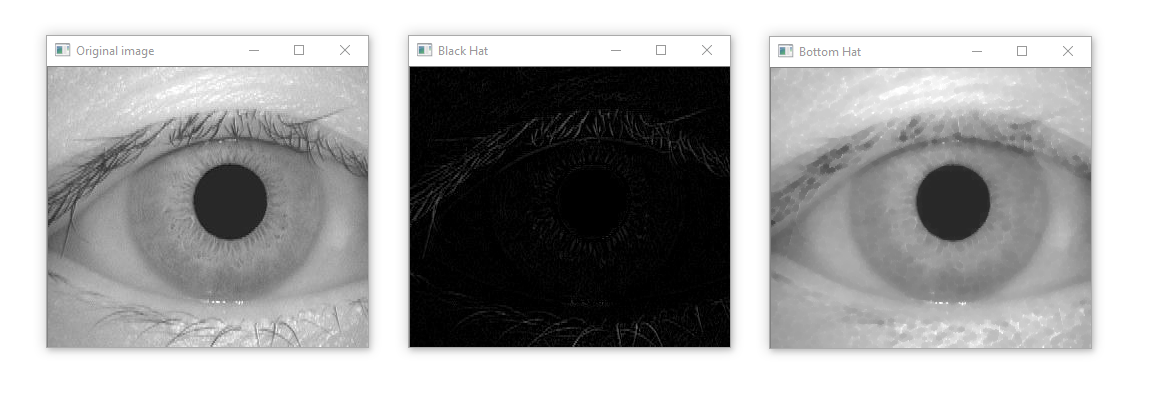
\includegraphics[width=1.0\textwidth]{black_hat}
  \caption{Applicazione della trasformazione black hat all'immagine}
\end{figure}

La scelta di queste trasformazioni morfologiche risiede nel fatto che si adattano molto bene alla successiva applicazione di un blur, in particolar modo del Gaussian Blur.

  \subsection{Gaussian Blur}
  Il filtro più importante è il Gaussian Blur, che prende in input: l’immagine filtrata dal black hat, un kernel (standard 5x5, che può essere eventualmente modificato con valori positivi dispari), una deviazione standard del kernel sigmaX e una sigmaY, nel nostro caso entrambe settate a 0 per farle calcolare automaticamente dalla funzione sulla base dei valori del kernel. 

\begin{minted}
  [
    xleftmargin=\parindent,
    framesep=2mm,
    baselinestretch=1.2,  
    fontsize=\footnotesize,
    linenos
  ]
  {python}
  
  final_img = cv2.GaussianBlur(bottom_hat_filtered, (5, 5), 0)   
  \end{minted}
  

In termini di elaborazione delle immagini, eventuali spigoli netti vengono uniformati, riducendo al minimo le sfocature. In questo caso l’utilità di questo filtro è quella di “pulire” ulteriormente l’immagine dell’occhio, semplificando la successiva identificazione della pupilla e,soprattutto, dell’iride.

\begin{figure}[t]
  \centering
  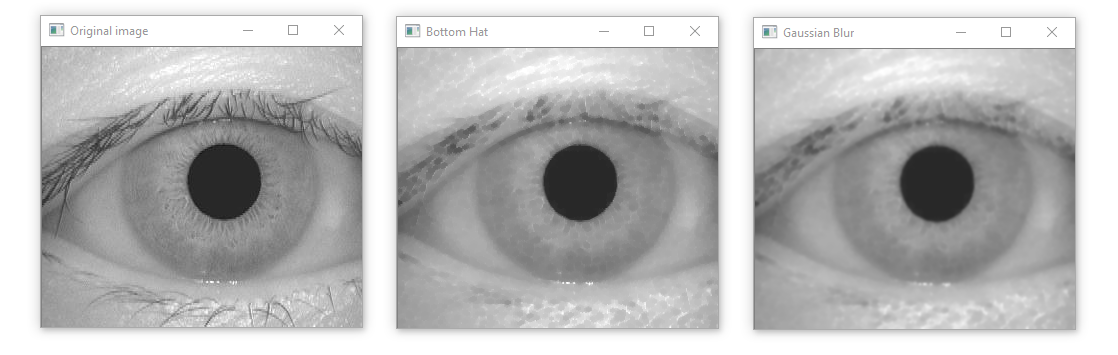
\includegraphics[width=1.0\textwidth]{gaussian_blur.png}
  \caption{Risultato dell'applicazione del Gaussian Blur dopo il filtro bottom hat}
\end{figure}

  \subsection{Sharpening filter / Correzione Gamma / Incremento luminosità}
  Sono stati inseriti all’interno di \texttt{filtering.py} (ma non utilizzati) tre filtri opzionali, essi possono essere abilitabili tramite gli omonimi parametri presenti nel file di configurazione alla sezione \texttt{FILTERING\_PUPIL/FILTERING\_IRIS}:

\begin{itemize}
  \item \textbf{Sharpen}: risalta i contorni nel caso in cui le immagini a disposizione siano di bassa risoluzione
  \item \textbf{Adjust\_Gamma}: modifica la gamma dell’immagine sulla base del parametro \texttt{GAMMA\_VALUE} (float)
  \item \textbf{Increase\_Brightness}: modifica la luminosità dell’immagine sulla base del parametro \texttt{BRIGHTNESS\_VALUE} (int)
\end{itemize}

  \subsection{Threshold}
  Dopo una prima applicazione dei filtri sopra descritti, si passa all’applicazione di un threshold tramite la funzione \texttt{cv2.threshold} della libreria OpenCV. Il suo funzionamento è semplice: essa prende in input un’immagine in grayscale ed effettua un confronto tra i valori dei singoli pixels e un valore di soglia. Considerando un caso binario, se il valore di un pixel è maggiore del valore di soglia, viene assegnato un valore specifico al pixel stesso (bianco o nero), altrimenti viene assegnato il valore opposto.

\begin{minted}
  [
    xleftmargin=\parindent,
    framesep=2mm,
    baselinestretch=1.2,  
    fontsize=\footnotesize,
    linenos,
    breaklines
  ]
  {python}
  
  def threshold(img, tValue, adaptive=False, binaryInv=False, otsu=False, dilate=False):
    if adaptive is False and otsu is False:
        _, thresh = cv2.threshold(img, tValue,
                                  255, cv2.THRESH_BINARY_INV if binaryInv else cv2.THRESH_BINARY)
    elif adaptive is True and otsu is False:
        thresh = cv2.adaptiveThreshold(
            img, 255, cv2.ADAPTIVE_THRESH_MEAN_C, cv2.THRESH_BINARY, 9, 1)
    elif adaptive is False and otsu is True:
        ret, thresh = cv2.threshold(
            img, 0, 255, cv2.THRESH_BINARY_INV + cv2.THRESH_OTSU)
    else:
        thresh = img

    if dilate is True:
        thresh = dilate_thresh(thresh)

    return thresh
    
\end{minted}

La funzione applica diversi threshold in base ai parametri scelti; nel caso dell’identificazione dell’iride si è scelto di applicare un threshold binario (default della funzione) all’immagine filtrata, il quale assegna ad un pixel il valore 255 (bianco) se il valore attualmente presente nel pixel è maggiore della soglia identificata dal parametro tValue. Per il caso in esame il valore di soglia ottimale è risultato essere 160.

\begin{figure}[h]
  \centering
  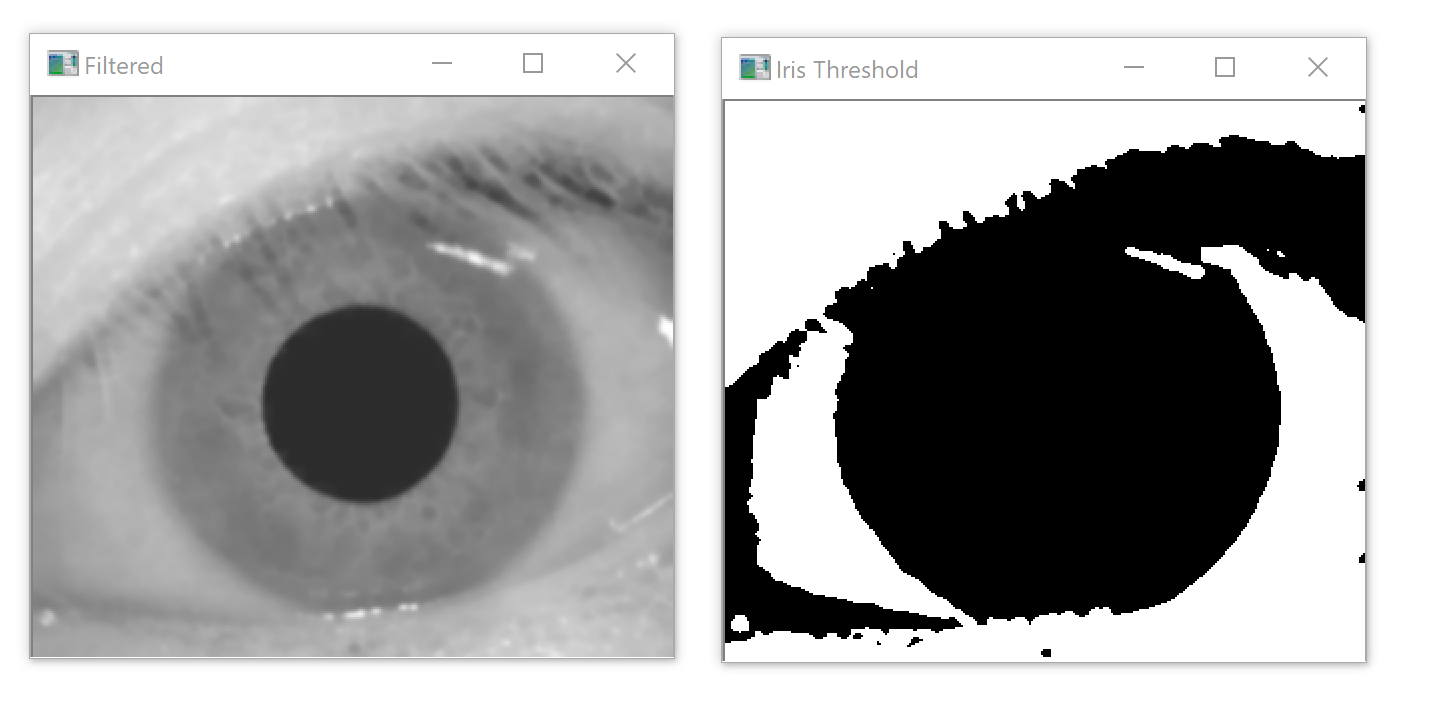
\includegraphics[width=1.0\textwidth]{threshold_iris.png}
  \caption{Applicazione del threshold binario per la delineazione dell'iride}
\end{figure}

Grazie a questo tipo di elaborazione si mette in risalto l’area dell’iride in modo da facilitare ulteriormente il successivo riconoscimento della circonferenza. 

Per il riconoscimento della pupilla si è utilizzato invece  un approccio simile, invece di applicare un classico threshold binario si è scelto di usare un threshold binario invertito, abilitando il parametro \texttt{BINARY\_INV}. L’unica differenza rispetto al threshold normale è che viene assegnato il valore 255 ai pixel minori del valore di soglia. La scelta è stata fatta perchè è risultato più performante utilizzare questo tipo di threshold per identificare l’area della pupilla, composta da pixel il cui valore di colore si avvicina di più allo 0 (nero). Il valore di soglia ottimale è risultato essere 70.

\begin{figure}[h]
  \centering
  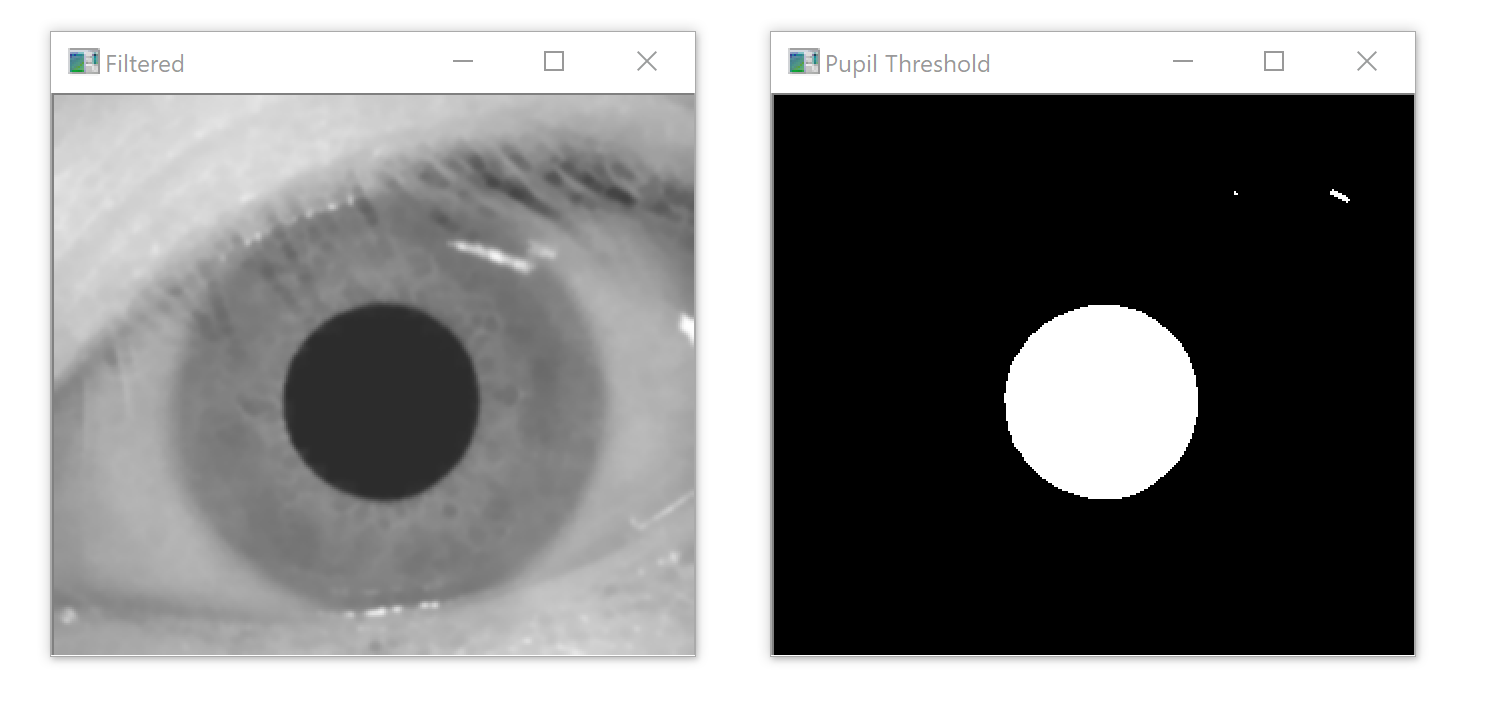
\includegraphics[width=1.0\textwidth]{threshold_pupil.png}
  \caption{Applicazione del threshold binario invertito per la delineazione della pupilla}
\end{figure}

La funzione di cui sopra prevede anche l’utilizzo di threshold diversi in base allo specifico impiego, essi sono attivabili modificando i relativi parametri presenti nelle sezioni \texttt{THRESHOLD\_PUPIL} e \texttt{THRESHOLD\_IRIS} del file di configurazione:

\begin{itemize}
  \item \textbf{Adaptive Threshold}: l’algoritmo calcola il threshold analizzando piccole regioni dell’immagine, ottenendo quindi diversi valori di soglia per diverse regioni. Si utilizza per immagini ad alto contrasto
  \item \textbf{Otsu Threshold}: l’algoritmo calcola in automatico il valore di soglia ottimale sulla base dell’istogramma dell'immagine
  \item \textbf{Dilate Threshold}: applica una trasformazione morfologica di dilatazione all’immagine ottenuta da una delle metodologie precedenti. L’utilità sarebbe quella di “riempire” i buchi
\end{itemize}

Nonostante fossero implementate tecniche di thresholding più avanzate, come Adaptive e Otsu, si è rivelato ottimale utilizzare il threshold binario normale e binario invertito in quanto gli algoritmi di identificazione di iride e pupilla si basano sul riconoscimento di cerchi nelle immagini, infatti con queste trasformazioni si vanno ad evidenziare maggiormente i cerchi delineati dall’iride e dalla pupilla.

  \subsection{Canny Edge Detection}
  L’algoritmo di Canny è uno dei più popolari algoritmi di riconoscimento dei contorni. L’algoritmo punta a trovare il maggior numero di contorni nell’immagine vicini ai contorni reali evitando di marcare più volte lo stesso contorno ed evitando di provocare falsi riconoscimenti.

E’ un algoritmo multi-stadio che si articola in 4 fasi:
\begin{enumerate}
  \item Riduzione del rumore
  \item Ricerca del gradiente della luminosità di un'immagine
  \item Soppressione dei non-massimi
  \item Individuazione dei contorni mediante sogliatura con isteresi
\end{enumerate}

Nella libreria OpenCV dell’algoritmo di Canny viene implementato dalla funzione \texttt{cv2.Canny}.

\begin{minted}
  [
    xleftmargin=\parindent,
    framesep=2mm,
    baselinestretch=1.2,  
    fontsize=\footnotesize,
    linenos,
    breaklines
  ]
  {python}
  
  canny = cv2.Canny(thresh, config.HOUGH_IRIS.getint(
   'CANNY_TH1'), config.HOUGH_IRIS.getint('CANNY_TH2'))   
\end{minted}

La funzione in automatico applica tutti e 4 gli stadi precedentemente citati, gli unici input obbligatori sono: l’immagine, che deve essere necessariamente in grayscale (single-channel), e due valori di soglia (chiamati threshold) per la procedura di isteresi. 

Nell'elaborato il Canny Edge viene utilizzato esclusivamente nella funzione di riconoscimento dell’iride, in particolare lo si applica all’immagine binaria (bianca e nera) ottenuta dalla precedente operazione di thresholding con i due parametri di soglia settati a 150 e 200 (\texttt{CANNY\_TH1} e \texttt{CANNY\_TH2}) . Si è scelto di utilizzarlo solo per la parte di riconoscimento dell’iride  in quanto il threshold di per sé non bastava a portare una buona accuratezza nel riconoscimento della circonferenza. Infatti, a differenza della pupilla che ha tutti i valori di pixel vicino al nero, per la parte dell’iride non esiste un valore di soglia che sia in grado di evidenziare la sola  area di iride in quanto ci possono essere delle parti dell’occhio, diversi dall’iride, con valori dei pixel inferiori alla soglia che vengono categorizzati come nero. La seguente immagine evidenzia questo problema, si nota infatti come, a differenza della pupilla, l’area di interesse dell’iride non venga perfettamente delineata.

\begin{figure}[h]
  \centering
  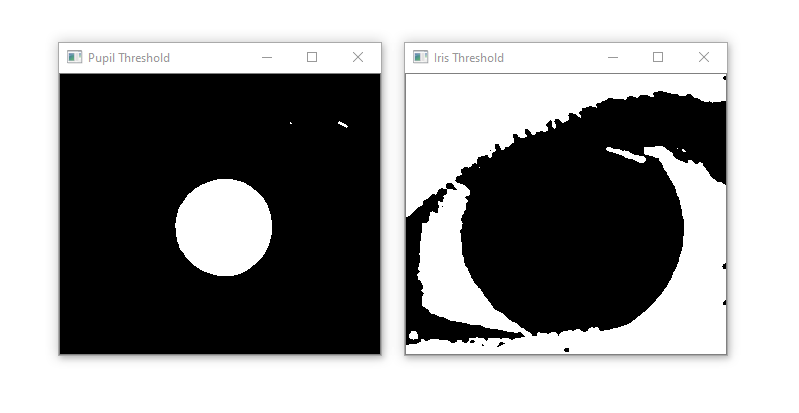
\includegraphics[width=1.0\textwidth]{canny_threshold.png}
  \caption{Confronto tra il risultato del threshold per iride e pupilla}
\end{figure}

Si è quindi ritenuto necessario applicare l’algoritmo di Canny al solo riconoscimento dell’iride in modo da definire il più possibile l’area di interesse, mentre per la pupilla non è risultato necessario applicare ulteriori trasformazioni.

\begin{figure}[h]
  \centering
  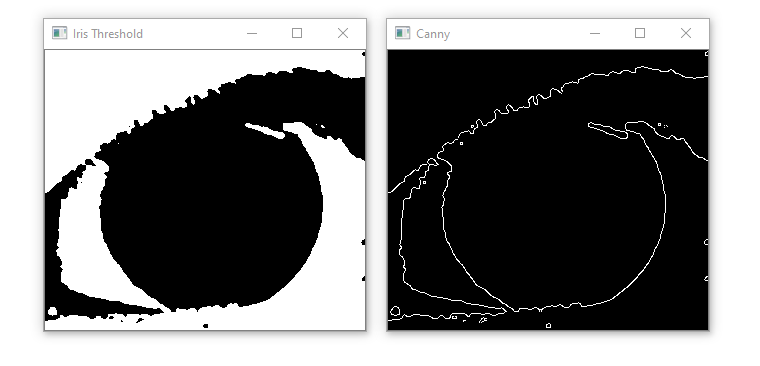
\includegraphics[width=1.0\textwidth]{canny_edge.png}
  \caption{Applicazione del Canny Edge Detector in successione al treshold}
\end{figure}

Il risultato ottenuto dal Canny Edge è quindi un’immagine in cui gran parte dei contorni dell’iride è ben definito e ciò risulta essere molto utile per il passo successivo ovvero l’identificazione di cerchi nell’immagine. Il Canny di fatto fornisce all’algoritmo di riconoscimento  già una buona parte della circonferenza dell’iride e di conseguenza risulterà anche più semplice ed accurato il riconoscimento della circonferenza completa.

  \section{Circle Hough Transform}
  La funzione più importante di tutta la sezione di elaborazione delle immagini  dell’occhio è quella di riconoscimento dei cerchi. Per far ciò si utilizza una delle più popolari tecniche in tale ambito, chiamata Circle Hough Transform (CHT); questa tecnica è una derivazione della trasformata di Hough, tecnica molto usata nel campo della computer vision, che consiste nell’estrazione di feature dalle immagini. La trasformata si basa sul riconoscimento di linee, tuttavia è stata estesa anche al riconoscimento di forme geometriche, in questo caso la CHT è l’estensione della trasformata di Hough per il riconoscimento dei cerchi, concentrandosi sulle coordinate del centro e al raggio. Per il caso in esame il raggio è a priori sconosciuto, l'algoritmo quindi lavora in uno spazio tridimensionale di parametri (composto dalle coordinate del centro e raggio), i parametri di un certo cerchio possono essere identificati dall’intersezione di più superfici coniche definite dai punti della circonferenza nello spazio 2D. Tale processo può essere suddiviso in due passi. Nel primo si trova ed eventualmente si perfeziona la misura del raggio, successivamente si ricava il centro ottimale dei cerchi in uno spazio bidimensionale dei parametri. Nel secondo passo invece si cerca di trovare il raggio ottimale in uno spazio monodimensionale dei parametri. Viene utilizzata una matrice di accumulazione, chiamata accumulatore, tridimensionale in quanto lo spazio originale dei parametri è 3D. Vengono poi iterati i possibili raggi, applicando i due passi sopra descritti.
 
Internamente l’algoritmo per arrivare a decidere quali sono i cerchi dell’immagine opera in diverse fasi: vengono applicati filtri di blur Gaussiano all’immagine convertita in grayscale, si definisce poi un operatore per il Canny Edge interno la funzione, il quale definisce i contorni, successivamente nell’accumulatore vengono valutati tutti i possibili cerchi, quelli scelti dall’algoritmo a partire dall’accumulatore definiscono il Circle Hough Space, all’interno del quale il cerchio più “votato” è quello ritenuto reale.

Nel codice, per implementare la CHT, si è usata la funzione \texttt{cv2.HoughCircles} fornita dalla libreria OpenCV; data un'immagine in input e specificati gli opportuni parametri la funzione restituisce una terna (X,Y,R), formata dalla coordinata X del centro, dalla coordinata Y del centro e raggio per ogni circonferenza identificata. E’ importante menzionare il fatto che, nonostante tutto il processo di calcolo dei parametri del cerchio venga svolto semplicemente invocando la funzione, la trasformata di per sé risulta essere un processo abbastanza dispendioso in termini di memoria e capacità computazionale, perciò gli sviluppatori della libreria OpenCV hanno scelto di implementare una variante della CHT standard chiamata Hough Gradient Method.

\begin{minted}
  [
    xleftmargin=\parindent,
    framesep=2mm,
    baselinestretch=1.2,  
    fontsize=\footnotesize,
    linenos,
    breaklines
  ]
  {python}
  
  circles = cv2.HoughCircles(
   thresh, cv2.HOUGH_GRADIENT, config.HOUGH_PUPIL.getfloat(
       'INVERSE_RATIO'), image.shape[0],
   param1=config.HOUGH_PUPIL.getint('PARAM1'), param2=config.HOUGH_PUPIL.getint('PARAM2'),
   minRadius=config.HOUGH_PUPIL.getint('MIN_RADIUS'), maxRadius=config.HOUGH_PUPIL.getint('MAX_RADIUS'))   
\end{minted}

Nel caso in esame viene passata come immagine in input l’immagine risultato dell’applicazione del threshold (nel caso del riconoscimento dell’iride è quella successiva all’applicazione del Canny Edge) mentre per quanto riguarda l’identificazione dei cerchi nell’immagine di un occhio si è interessati al rilevamento di un unico cerchio per pupilla e iride; per far ciò si è dovuto cercare i parametri della trasformata in modo da ridurre al minimo i possibili falsi (o multipli) ritrovamenti nel dataset utilizzato.

I parametri fondamentali della funzione sono:
\begin{itemize}
  \item \textbf{INVERSE\_RATIO}: rapporto inverso tra la risoluzione dell'accumulatore e la risoluzione dell'immagine. Ad esempio se vale 2 l’accumulatore è ampio la metà della risoluzione dell’immagine. Il parametro scelto è 0.8
  \item \textbf{MIN\_DIST}: distanza minima tra i centri di due cerchi individuati. Se il parametro è troppo piccolo si potrebbero riscontrare falsi riconoscimenti mentre se è troppo grande si potrebbero mancare alcuni cerchi reali. Si è scelto di settare il parametro al valore di height dell’immagine (\texttt{image.shape[0]})
  \item \textbf{PARAM\_1}: è il valore di soglia maggiore per il Canny Edge interno, il valore più piccolo invece è due volte minore di quello più alto. Il valore scelto è 20 per la pupilla e 30 per l’iride
  \item \textbf{PARAM\_2}: valore di threshold dell’accumulatore per la ricerca dei centri dei cerchi. Un valore più piccolo porta ad numero più alto di riconoscimenti (potenzialmente anche falsi) mentre un valore più alto porta ad un numero inferiore di riscontri ma questi riscontri hanno una probabilità maggiore di essere corretti. Per la pupilla si è utilizzato il valore 5 mentre per l’iride il valore 10
  \item \textbf{MIN\_RADIUS}: raggio minimo dei cerchi. Per la pupilla si è scelto il valore 18 mentre per l’iride il valore 90
  \item \textbf{MAX\_RADIUS}: raggio massimo dei cerchi. Per la pupilla si è scelto il valore 60 mentre per l’iride il valore 130
\end{itemize}

Con questi parametri si rileva esattamente un cerchio per pupilla e iride per l’intero dataset di immagini, inoltre i cerchi rilevati sono, nella quasi totalità dei casi, abbastanza accurati rispetto alle reali circonferenze di iride e pupilla.

\begin{figure}[h]
  \centering
  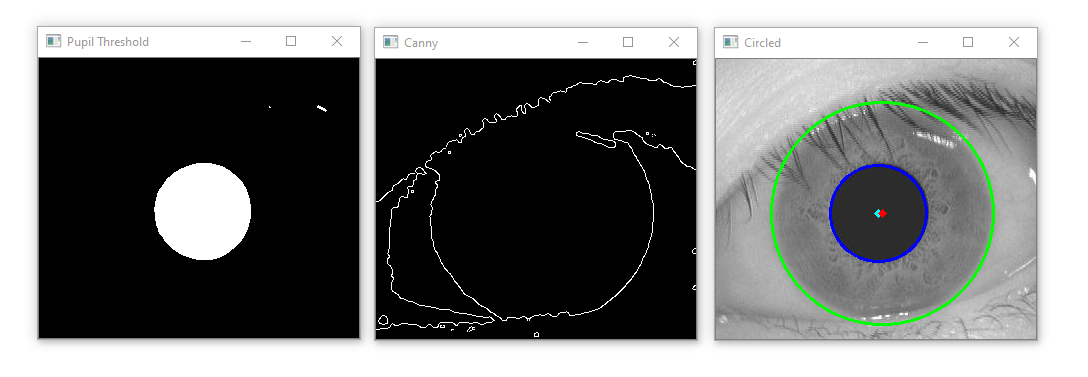
\includegraphics[width=1.0\textwidth]{hough.png}
  \caption{Esito dell'applicazione della funzione \texttt{cv2.HoughCircles}}
\end{figure}

\emergencystretch 5em%

Le funzioni \texttt{pupil\_recognition} e \texttt{iris\_recognition} presenti in \texttt{preprocessing.py}, ovvero le funzioni che si occupano di richiamare tutte le varie tecniche di elaborazione dell’immagine, terminano con l’Hough Circles Transform e quindi restituiscono in output i  valori di centro e raggio del cerchio trovato, tali valori verranno poi utilizzati nella successiva fase di segmentazione. Nel caso in cui invece non vengano trovati cerchi, oppure ne vengano trovati più di uno per iride e pupilla, l’immagine causa dei problemi viene scartata, quindi non sarà più considerata nell’insieme di immagini di training in quanto non potrà essere segmentata.

  \section{Segmentazione}
  Una volta identificati i cerchi di iride e pupilla e salvati i relativi parametri di centro e raggio in due vettori, rispettivamente chiamati \texttt{iris\_circle} e \texttt{pupil\_circle}, si passa alla segmentazione vera e propria, nella quale viene isolata la regione di interesse dell’iride. A tale scopo è stata definita una funzione all’interno di \texttt{processing.py} denominata segmentation:

\begin{minted}
  [
    xleftmargin=\parindent,
    framesep=2mm,
    baselinestretch=1.2,  
    fontsize=\footnotesize,
    linenos,
    breaklines
  ]
  {python}
  
  def segmentation(image, iris_circle, pupil_circle, startangle, endangle, min_radius, max_radius)  
\end{minted}

La funzione prende in input i vettori dei parametri dei cerchi, \texttt{iris\_circle} e \texttt{pupil\_circle}, un angolo di partenza, uno di fine e due valori limite di raggio. Per adattare il codice ad ogni tipo di dimensione si è utilizzato un approccio particolare, basato sull’uso di percentuali. In questo modo è possibile ottenere porzioni intermedie di iride indicando la percentuale minima e massima del raggio totale che si vuole considerare. I valori percentuali di default sono 0\% e 100\% in modo da prendere l’intera iride, quindi partendo dal bordo della pupilla (identificato dal suo raggio) ed arrivando fino al bordo esterno, tuttavia risultano modificabili tramite i parametri \texttt{MIN\_RADIUS} e \texttt{MAX\_RADIUS} della sezione \texttt{PREPROCESSING} del file di configurazione. Nel caso di inserimento di valori fuori limite verranno in automatico utilizzati i valori di default.

\begin{minted}
  [
    xleftmargin=\parindent,
    framesep=2mm,
    baselinestretch=1.2,  
    fontsize=\footnotesize,
    linenos,
    breaklines
  ]
  {python}
  
  outer_sector = np.zeros((height, width), np.uint8)
  inner_sector = np.zeros((height, width), np.uint8)

  if min_radius < max_radius:
      draw_ellipse(outer_sector, (iris_circle[0], iris_circle[1]), (
          max_radius, max_radius), 0, -startangle, -endangle, 255, thickness=-1)
      cv2.circle(inner_sector, (pupil_circle[0], pupil_circle[1]), int(
          min_radius), 255, thickness=-1)
  mask = cv2.subtract(outer_sector, inner_sector)
  masked_image = cv2.bitwise_and(segmented, segmented, mask=mask)

  return masked_image, mask 
\end{minted}

Il funzionamento è semplice: si inizializzano delle maschere, rappresentate da delle matrici di zeri della stessa dimensione dell’immagine originale (immagini nere), in questo caso chiamate \texttt{outer\_sector} e \texttt{inner\_sector}. Le maschere sono un modo per selezionare parti specifiche di immagini, in sostanza si vanno a marcare i pixel che si vogliono considerare mettendo a 1 i valori nelle rispettive posizioni nella maschera. Facendo l’AND logico tra la maschera e l’immagine originale si ottengono solo i pixel corrispondenti alla parte desiderata dell’immagine. Si utilizzano quindi i parametri di \texttt{iris\_circle} e \texttt{pupil\_circle} e quelli definiti dall’utente nella chiamata alla funzione per creare due maschere. La prima consiste in un settore circolare con raggio uguale al raggio massimo definito precedentemente. Essa viene ottenuta grazie alla funzione \texttt{draw\_ellipse}, si crea poi la seconda maschera, corrispondente ad un cerchio di raggio minimo (se 0\% il cerchio corrisponde alla pupilla) tramite la funzione \texttt{cv2.circle}. Successivamente, tramite la funzione di OpenCV \texttt{cv2.subtract} si crea un’unica maschera finale contenente i pixel ottenuti dalla dalla sottrazione tra \texttt{outer\_sector} e \texttt{inner\_sector}, ottenendo così la maschera relativa all’area di interesse. Infine l’area di interesse vera e propria è ricavata tramite la funzione \texttt{cv2.bitwise\_and}, la quale effettua una AND tra l’immagine di partenza e l’ultima  maschera creata, ottenendo così i soli pixel reali del segmento di iride.

\begin{figure}[h]
  \centering
  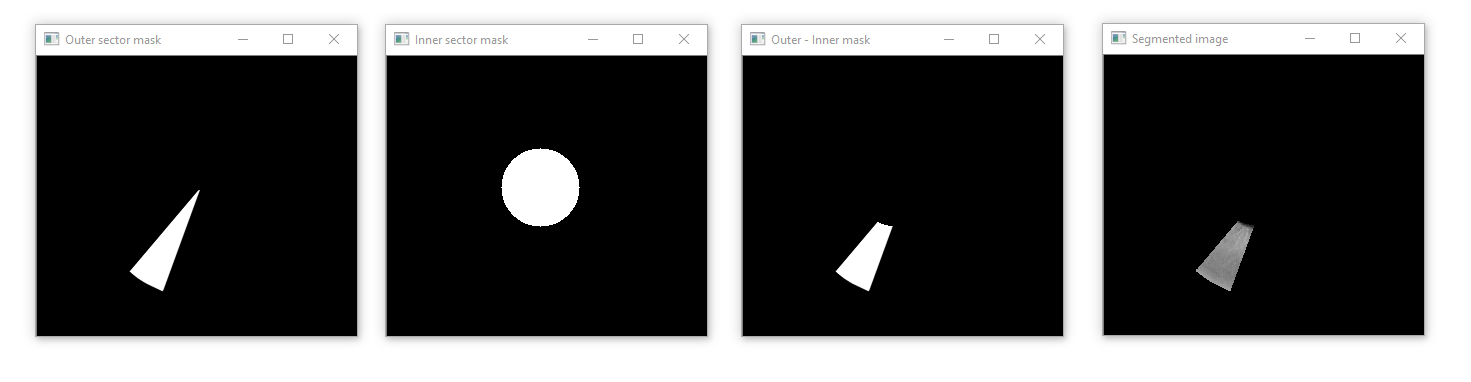
\includegraphics[width=1.0\textwidth]{segmentazione.png}
  \caption{Segmentazione dell'iride per ottenere la regione d'interesse}
\end{figure}

  \section{Crop, Resize e salvataggio}
  Una volta isolati i segmenti di iride d’interesse dall’immagine originale si può procedere all’ultima fase di questa sezione di elaborazione delle immagini. Come si è visto prima, la fase di segmentazione produce un’immagine completamente a sfondo nero tranne nella parte in cui è presente la regione di interesse. L’elevata presenza di pixel neri, i quali non contengono informazioni utili,  potrebbe “confondere” la rete neurale, la quale darebbe pesi errati alle sezioni nere. Risulta quindi necessario ritagliare l’immagine in modo tale da valorizzare al massimo i pixel effettivamente utili, ovvero quelli del segmento. Tale operazione si chiama cropping e la funzione seguente ne è l’implementazione:

\begin{minted}
  [
    xleftmargin=\parindent,
    framesep=2mm,
    baselinestretch=1.2,  
    fontsize=\footnotesize,
    linenos,
    breaklines
  ]
  {python}
  
  def crop_image(masked_image, offset=30, tollerance=80):
   mask = masked_image > tollerance
   coords = np.argwhere(mask)
   x0, y0 = coords.min(axis=0)
   x1, y1 = coords.max(axis=0) + 1  # slices are exclusive at the top
   cropped = masked_image[x0 - offset: x1 + offset, y0 - offset: y1 + offset]
   return cropped  
\end{minted}

La funzione restringe l’immagine attorno ai pixel non neri, quindi quelli definiti dal segmento di iride, riducendo al minimo possibile il nero senza eliminare i pixel contenenti l’informazione utile.

\begin{figure}[h]
  \centering
  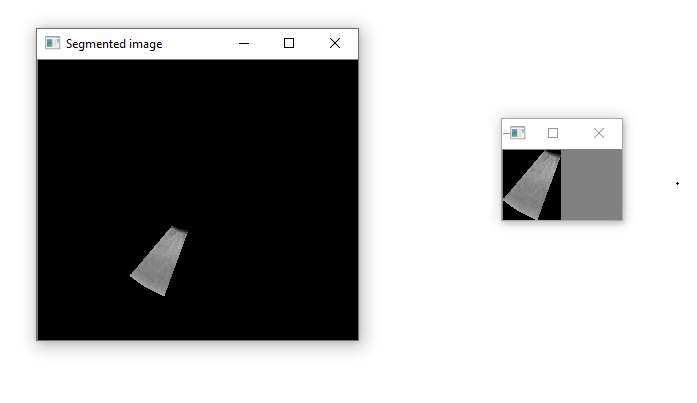
\includegraphics[width=1.0\textwidth]{crop.png}
  \caption{Operazione di cropping dell'immagine}
\end{figure}

Al termine di questo passaggio si ottengono quindi immagini relativamente piccole nel quale la maggior parte dei pixel rappresenta la regione di interesse.

A questo punto il dataset per il training è quasi pronto, tuttavia prima bisogna risolvere un problema introdotto dal cropping. Anche partendo da immagini della stessa dimensione i vari segmenti d’iride possono risultare di dimensione diversa in quanto le naturali conformazioni dell’occhio umano non sono mai perfettamente uguali, quindi il cropping su questi segmenti potrebbe produrre immagini di dimensione diversa. Immagini a dimensione non uniforme non vanno bene per una CNN in quanto nel processo di training essa si aspetta in input matrici (rappresentazione interna delle immagini) tutte della stessa dimensione. Per risolvere questo problema si è implementato un meccanismo di resize automatico delle immagini dei segmenti alla loro dimensione media.

\begin{minted}
  [
    xleftmargin=\parindent,
    framesep=2mm,
    baselinestretch=1.2,  
    fontsize=\footnotesize,
    linenos,
    breaklines
  ]
  {python}
  
  def get_average_shape(cropped_dict):
   shapes = np.concatenate(([c.shape for c in cropped_dict['DB_PROBS']], [c.shape for c in cropped_dict['DB_NORMAL']]))
   means = np.around(np.mean(shapes, axis=0)).astype(int)
   return means 
\end{minted}

Utilizzando la funzione sopra citata si calcolano height e width medie tra tutte le immagini risultanti dalla fase di cropping,  poi si procede, tramite la funzione \texttt{cv2.resize} di OpenCV, al ridimensionamento di tali immagini alle dimensioni trovate. E’ vero che un resize potrebbe portare ad una riduzione della qualità dell’immagine (ad esempio un ingrandimento risulterebbe in un'immagine sgranata) tuttavia le dimensioni ottenute dopo il cropping risultano molto vicine tra di loro quindi un resize alla dimensione media non comporta una grossa perdita di qualità.

A questo punto si è definitivamente pronti per la fase di training; lo script \texttt{preprocess.py} termina con il salvataggio delle immagini croppate e ridimensionate nella cartella \texttt{TEMP\_SEG}; vengono poi suddivise in due sotto cartelle, \texttt{DB\_NORMAL\_SEG} e \texttt{DB\_PROBS\_SEG}, in relazione alla loro sottocartella di \texttt{DATA\_IMAGES} di provenienza.

  
  \chapter{Processo di sviluppo di un modello di rete neurale per applicazioni all'iridologia}
  \section{Data Preparation}
  Una volta estratti i segmenti di iride dalle immagini originali dell’occhio si può passare alla fase di training. La vera e propria fase di training tuttavia necessita di due prerequisiti: la fase di preparazione dei dati e la fase di creazione del modello. Avviando lo script \texttt{train.py} la prima operazione che viene eseguita è quindi quella di preparazione dei dati, a tale scopo si invoca la funzione \texttt{create\_trainig\_data} presente nel file \texttt{data\_preparation.py} contenuto nel modulo \texttt{ML\_CNN}; in sostanza la funzione si occupa di strutturare i dati in modo tale che possano essere correttamente recepiti dalla rete neurale. Si parte caricando le immagini dei segmenti in memoria, già in fase di caricamento ad ogni immagine viene associata una label ovvero un identificatore che poi la rete utilizzerà per categorizzare le immagini. Si scorre quindi tra le immagini presenti nelle due sottocartelle di \texttt{TEMP\_SEG}  e per ogni immagine si crea un array contenente la matrice dei pixel che rappresenta l’immagine e la label di riferimento, in particolare se l’immagine proviene dalla sottocartella \texttt{DB\_NORMAL\_SEG} viene assegnata la label 0, ad indicare che il segmento non presenta problematiche, nel caso contrario invece si assegna la label 1. 

Ogni vettore matrice-label viene poi aggiunto in coda ad un altro vettore chiamato \texttt{training\_data}, tale vettore una volta finite le iterazioni conterrà tutte le coppie immagini-label. Successivamente su questo vettore si effettua uno shuffle ovvero si cambia l’ordine dei vari elementi interni;  ciò risulta molto utile nella fase training in quanto in questo modo la rete evita di imparare eventuali pattern nella distribuzione dei dati stessi e quindi si evita l’introduzione di una possibile distorsione nella previsione finale. Dopo lo shuffle si procede alla creazione di due particolari vettori:

\begin{itemize}
  \item \textbf{Features}: le features sono le variabili indipendenti che agiscono come input del modello. Il modello impara dalle features per poi fare le previsioni
  \item \textbf{Labels}: le labels rappresentano l’output finale, le classi in cui categorizzare le immagini
\end{itemize}

Nel caso d’uso, il vettore delle features, comunemente chiamato \texttt{X}, contiene tutte le matrici di pixel (ovvero le immagini) presenti nell’array \texttt{training\_data}, mentre il vettore delle labels, detto \texttt{y}, contiene i valori di categorizzazione (0 o 1) associati ad ogni immagine. In sostanza quello che accade è che partendo dall’array \texttt{training\_data} si separano le immagini dalle label, la corrispondenza segmento-label viene mantenuta tramite l’indice di posizione nei rispettivi array. 

L’ultimo passaggio da fare prima di poter ottenere i dati nel formato corretto è quello di reshape dell’array \texttt{X} (array di feature). Tale passaggio è necessario in quanto il modello si aspetta un dataset di input della forma (numero di immagini, height dell’immagine, width dell’immagine, numero di canali dell’immagine), si effettua quindi un ridimensionamento, tramite la funzione \texttt{reshape} della libreria NumPy, sull’array \texttt{X} passando come ultimo parametro il valore 1 che sta ad indicare che si lavora con immagini a singolo canale, quindi grayscale. Dopo quest’ultimo passaggio si hanno i dati strutturati nella forma corretta per il training, i vettori necessari sono quindi \texttt{X} (features) e \texttt{y} (labels).

L’utente può inoltre, a sua scelta, abilitare il parametro \texttt{SAVE\_TRAIN\_DATA} nella sezione \texttt{NEURAL\_NETWORK\_TRAIN} per effettuare il salvataggio su disco dei vettori \texttt{X} e \texttt{y} in modo da poterli riutilizzare in futuro, ad esempio per fare training su reti diverse. Il salvataggio avviene grazie al modulo pickle (nativo in python 3) che si occupa di serializzare oggetti python in vettori di caratteri. I file risultanti dall serializzazione sono \texttt{X.pickle} e \texttt{y.pickle}. Per il training del modello vengono comunque utilizzati gli ultimi vettori di \texttt{X} e \texttt{y} prodotti.

  \section{Convolutional Neural Networks}
  Nell’ambito del deep learning, una convolutional neural network (CNN) è una branca delle deep neural networks, applicata più comunemente all’analisi e la riconoscimento di pattern nelle immagini. Le CNN sono ispirate da processi biologici nei quali il pattern di connettività dei neuroni somiglia a quello della corteccia visiva animale. Singoli neuroni rispondono solo a stimoli provenienti da una specifica regione del campo visivo. 

Una CNN è progettata in modo tale da utilizzare al minimo la pre-elaborazione, in quanto la rete impara da sola a gestire i suoi filtri e la loro applicazione, cosa che non può avvenire in altri algoritmi di riconoscimento delle immagini; le informazioni che passano per la rete influenzano la struttura stessa della CNN poiché una rete neurale cambia, o impara, in base agli input e agli output intermedi. Una CNN consiste infatti in un input layer, un output layer e molteplici layers intermedi, chiamati hidden layers. Questi ultimi possono essere di vario tipo, tipicamente per una CNN vengono utilizzati layers convoluzionali, layers di attivazione (es. RELU), pooling layers, dense layers e flatten layers. 

  \section{Il modello}
  Nell’ambito di questo progetto è stata scelta l’implementazione di una CNN relativamente standard, eventualmente ampliabile per progetti futuri. Viene utilizzata un modulo di Tensorflow chiamato Keras, grazie al quale possiamo strutturare il modello per poi andare ad analizzare le immagini dei segmenti di iride. 

La funzione che crea il modello è definita in \texttt{model.py} nel pacchetto \texttt{ML\_CNN} e si chiama \texttt{create\_model}.

\begin{minted}
  [
    xleftmargin=\parindent,
    framesep=2mm,
    baselinestretch=1.2,  
    fontsize=\footnotesize,
    linenos,
    breaklines
  ]
  {python}
  
  model = Sequential()
  model.add(Conv2D(layer_size, (3, 3), input_shape=X.shape[1:]))
  model.add(Activation('relu'))
  model.add(MaxPooling2D(pool_size=(2, 2)))

  for l in range(conv_layer - 1):
    model.add(Conv2D(layer_size, (3, 3)))
    model.add(Activation('relu'))
    model.add(MaxPooling2D(pool_size=(2, 2)))

  model.add(Flatten())

  for l in range(dense_layer):
    model.add(Dense(layer_size))
    model.add(Activation('relu'))  

  model.add(Dense(1))
  model.add(Activation('sigmoid'))

  model.compile(loss='binary_crossentropy',
                optimizer='adam',
                metrics=['accuracy'])

  return model, modelname 
\end{minted}

Il tipo di modello che viene utilizzato è quello sequenziale, per creare un modello di questo tipo basta creare un’istanza della classe \texttt{Sequential} di Keras. \texttt{Sequential} è il modo più semplice per costruire un modello, in quanto si definiscono i singoli hidden layers uno ad uno. 

Il primo layer che viene aggiunto è quello convoluzionale, \texttt{Conv2D} (input layer). Esso è a stretto contatto con l’input layer, operando sulle immagini in input, viste come matrici bidimensionali. L’argomento \texttt{layer\_size} indica il numero di neuroni che costituiranno il livello ed è possibile settare questo valore tramite il parametro \texttt{LAYER\_SIZE} della sezione \texttt{NEURAL\_NETWORK\_MODEL} del file di configurazione. Si scelgono solitamente valori standard come 32, 64, 128, etc... in base al numero di immagini presenti nel dataset. Va definita inoltre una kernel size, in questo caso lasciata standard, ovvero 3x3. Essa è la dimensione del kernel, una matrice di filtraggio necessaria alla convoluzione. Una convoluzione è un’operazione che trasforma una funzione matematica al fine di ricavarne maggiori informazioni. In ambito di computer vision, si va a trasformare la matrice rappresentate l’immagine attraverso i valori presenti nel kernel mediante una moltiplicazione matriciale. L’area in cui si trova il kernel viene chiamata receptive field, e in quest’area vengono pian piano applicati i filtri. Questi ultimi non sono definiti in una CNN, in quanto è la rete a imparare in fase di training la tipologia e i parametri di tali filtri. I filtri del layer \texttt{Conv2D} vengono applicati su tutta l’immagine mediante lo “scorrimento” del kernel. La scelta dei filtri che \texttt{Conv2D} applica è inizialmente casuale e basata su distribuzioni conosciute (normale, gaussiana, etc...), ogni filtro viene così trainato in modo differente dagli altri, imparando pian piano a riconoscere features particolari delle immagini. 

Successivamente viene aggiunto un activation layer, un livello che fa passare i dati in input attraverso una funzione di attivazione. Essa è una funzione matematica, possono essere utilizzate diverse funzioni in base al tipo di operazione che si deve effettuare in un determinato layer. Generalmente viene utilizzata la \texttt{RELU (Rectified Linear Unit)} come funzione di attivazione in seguito ad un \texttt{Conv2D} layer. Eventuali diverse funzioni di attivazione verranno citate in seguito.

\begin{figure}[h]
  \centering
  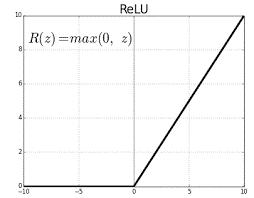
\includegraphics[scale=0.8]{relu.png}
  \caption{Grafico della funzione di attivazione Rectified Linear Unit}
\end{figure}

Viene poi aggiunto un Pooling layer, in particolare un \texttt{MaxPooling2D} layer. La ragione di ciò risiede nel fatto che questo tipo di livello opera un downsampling, riducendo il carico computazionale della rete, senza però perdere le informazioni importanti presenti nell’immagine, le quali vengono poi passate al layer successivo. Con il Max Pooling si considera solo il valore massimo tra tutti i pixel presenti nel kernel del filtro.

\begin{figure}[H]
  \centering
  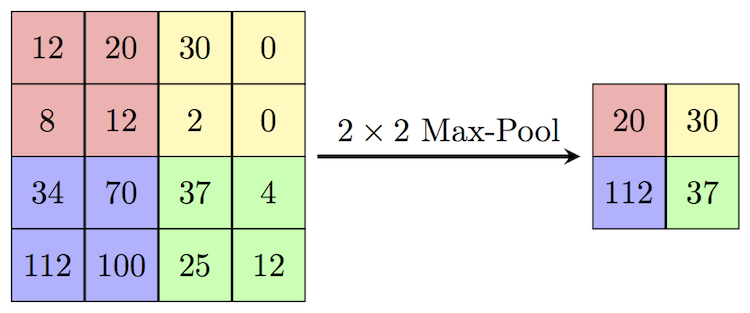
\includegraphics[scale=0.5]{pooling.png}
  \caption{Effetto del layer MaxPooling su un matrice bidimensionale}
\end{figure}

L’utente può poi impostare il valore del parametro \texttt{CONV\_LAYER} che indica il numero di volte in cui la terna di layers sopra descritta (Conv2D-Activation-MaxPooling2D) viene replicata. Così facendo si rende la rete parametrizzata, l’utente ha la possibilità di aggiungere o rimuovere layers intermedi a piacimento. 

Un altro layer molto importante è il \texttt{Flatten layer}. Non necessita di argomenti, in quanto esso si occupa solamente di “appiattire” un insieme di input in un unico vettore monodimensionale contenente tutti gli input. Ad esempio, se l’output del livello precedente ha una shape di (15, 15, 3), un flatten layer crea un vettore monodimensionale (15 x 15 x 3), in modo tale che possa poi essere preso in input da un \texttt{dense layer}. 

Un \texttt{dense layer} è un classico fully connected layer, in quanto ogni neurone è connesso a tutti gli altri. Anche in questo caso l’utente ha libertà di personalizzazione della rete, potendo decidere il numero di dense layers che vengono aggiunti in seguito al flatten layer modificando il parametro \texttt{DENSE\_LAYER}; anche il numero di neuroni dei dense layers è parametrizzabile mediante il parametro precedentemente citato, \texttt{LAYER\_SIZE}. La funzione di attivazione più adatta per questo tipo di layer intermedio rimane la \texttt{RELU}. 

Infine si aggiunge un ultimo \texttt{dense layer} (output layer), il quale si occuperà poi di dare il risultato finale, 0 e 1, essendo il problema in questione di tipo binario; la size di questo layer è 1 essendo che con un unico numero si coprono tutte le classi di categorizzazione (NORMAL e PROBS). La funzione di attivazione questa volta può essere scelta tra \texttt{Sigmoid} e \texttt{Softmax}; entrambe sono funzioni matematiche che si adattano bene al caso d’uso, ma la \texttt{Sigmoid} è scritta appositamente per un caso binario, mentre la \texttt{Softmax} per un caso multiclasse. Nulla sarebbe cambiato scegliendo la \texttt{Softmax} essendo uguali per un caso binario, una è la semplificazione dell’altra. 

\begin{figure}
  \centering
  \begin{subfigure}[b]{0.4\textwidth}
    \centering
    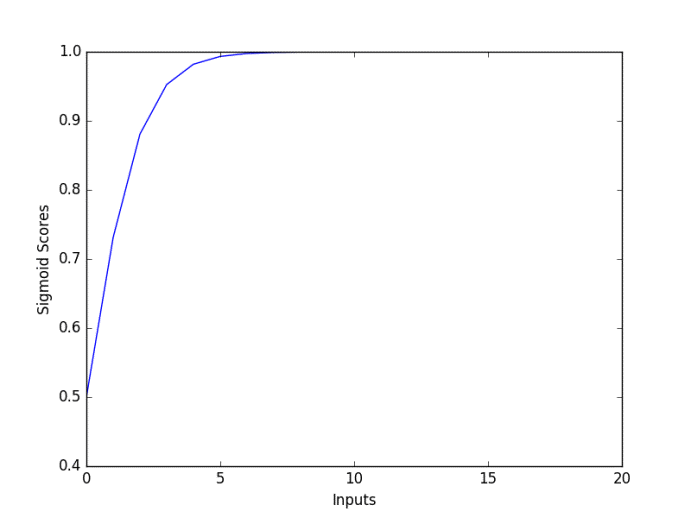
\includegraphics[width=\textwidth]{sigmoid.png}
    \caption{Sigmoid}    
  \end{subfigure}
  \hfill
  \begin{subfigure}[b]{0.4\textwidth}
    \centering
    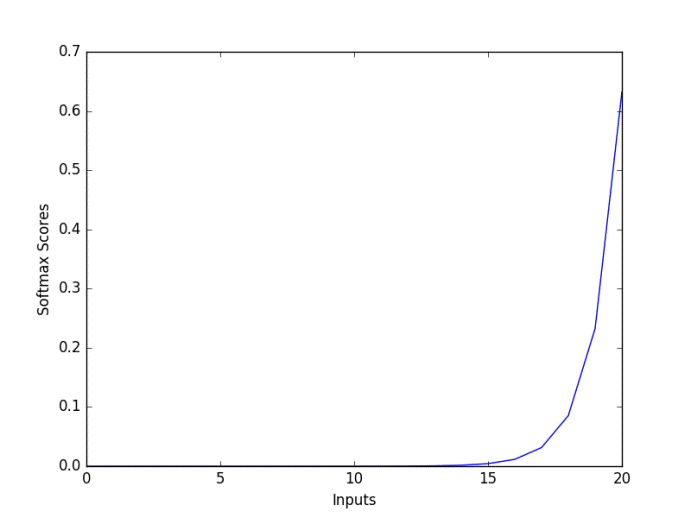
\includegraphics[width=\textwidth]{softmax.png}
    \caption{Softmax}       
  \end{subfigure}
  \caption{Grafici delle due principali funzioni di attivazione per l' ouput layer}
\end{figure}

Si conclude la strutturazione del modello tramite la funzione \texttt{compile} di Keras, la quale configura il modello, preparandolo per la successiva fase di training. I parametri \texttt{loss}, \texttt{optimizer} e \texttt{metrics} scelti sono abbastanza standard per un problema di tipo binario. La funzione di \texttt{loss} è necessaria in quando deve essere costantemente monitorato l’errore dello stato corrente del modello. In questo modo viene analizzato il \texttt{loss rate} in ogni layer, cercando di ridurlo nei layer successivi, aggiustando i pesi utilizzati per le varie operazioni nei livelli. Come metrica viene scelta \texttt{accuracy} in quanto si vuole verificare l’accuratezza del modello in percentuale. Una percentuale alta di \texttt{accuracy} e una bassa di \texttt{loss} indicano che il modello produce risultati attendibili e può essere quindi utilizzato con una buona confidenza per fare predizioni. Il modello viene infine ritornato alla funzione chiamante ed è pronto per la fase di training.

  \section{Training}
  A questo punto i prerequisiti fondamentali sono soddisfatti, si è creata la struttura della rete (contenuta nell’oggetto chiamato model) e i dati di input sono organizzati nel modo corretto, si è quindi pronti per il training vero e proprio. Nello script \texttt{train.py} alla terminazione della funzione \texttt{create\_model} viene invocata la funzione \texttt{train\_model}.

\begin{minted}
  [
    xleftmargin=\parindent,
    framesep=2mm,
    baselinestretch=1.2,  
    fontsize=\footnotesize,
    linenos,
    breaklines
  ]
  {python}
  
  def train_model(model, modelname, X, y, batch_size=32, epochs=3, validation_split=0.3, tensorboard=True):
   MODELDIR = './MODELS'
   LOGDIR = os.path.join(MODELDIR, 'LOGS')
   if not os.path.exists(MODELDIR):
       os.makedirs(MODELDIR)
   std_X = X / 255.0
   if tensorboard is True:
       if not os.path.exists(LOGDIR):
           os.makedirs(LOGDIR)

       tensorboard = TensorBoard(log_dir=os.path.join(LOGDIR, modelname))
       model.fit(std_X, y, batch_size=batch_size, epochs=epochs, validation_split=validation_split,
                 callbacks=[tensorboard])
   else:
       model.fit(std_X, y, batch_size=batch_size, epochs=epochs, validation_split=validation_split)

   model.save(os.path.join(MODELDIR, modelname)) 
\end{minted}

La funzione prende in input i vettori di features e labels (\texttt{X} e \texttt{y}), il modello ed altri parametri legati al training. Per prima cosa si effettua una normalizzazione di tutti i pixel di tutte le immagini contenuti nel vettore \texttt{X}, in questo modo si ottengono valori di pixel compresi tra 0 e 1. La normalizzazione è effettuata semplicemente dividendo per 255 tutti i pixel, dato che rappresenta il valore massimo che un pixel può avere. 

Dopo la normalizzazione si chiama il metodo \texttt{fit} sul modello, tale metodo è una funzione richiamabile da ogni modello creato con Tensroflow/Keras. \texttt{Fit} oltre ai vettori \texttt{X} (normalizzato precedentemente) e \texttt{y} prende in input alcuni importanti parametri:

\begin{itemize}
  \item \textbf{Epochs}: è un parametro che definisce il numero di volte in cui l’algoritmo di apprendimento attraverserà l’intero dataset di input. In sostanza un epoch è una iterazione dell’intero dataset composto dai vettori \texttt{X} e \texttt{y}
  \item \textbf{Batch Size}: definisce il numero di campioni da analizzare prima di fare un update dei parametri interni (default 32). Sostanzialmente si itera sul numero di campioni specificati da \texttt{batch size}, a fine iterazione si fanno delle prediction ed i risultati sono comparati con i valori previsti dell’output. Si calcola quindi l’errore e tramite esso l’algoritmo di apprendimento modifica i parametri interni per migliorare il modello
  \item \textbf{Validation Split}: decimale compreso tra 0 e 1, rappresenta la frazione del training set che verrà utilizzata per validare le performance del modello. Il modello terrà da parte questa frazione di dati e non li utilizzerà per il training. Verranno usati alla fine di ogni \texttt{epoch} per calcolare il \texttt{loss} e \texttt{l’accuratezza di validazione}  
\end{itemize}

A questo punto l’algoritmo di apprendimento inizia. Una volta terminato, la funzione \texttt{train\_model}, precedentemente definita, salva su disco nella cartella \texttt{MODELS} il modello appena trainato in modo da poterlo utilizzare in seguito per la fase di prediction. 

E’ importante far notare il fatto che la fase di training di un modello di rete neurale è un compito computazionalmente complesso e quindi il tempo di attesa per la terminazione del training può variare a seconda di diversi fattori: complessità stessa della rete, numero di epochs, training eseguito su CPU o GPU, numero di dati, etc… E’ quindi consigliato l’uso di uno strumento di analisi dei modelli, chiamato Tensorboard, che permette di analizzare i risultati del modello appena trainato in modo da ridurre il numero di operazione di training da fare per ottenere i risultati desiderati.


  \section{Tensorboard}
  Dato che creare e trainare un buon modello di machine learning non è semplice, nell’elaborato è stato inserito il supporto di una piattaforma per la progettazione e lo studio di modelli, tale applicativo si chiama Tensorboard.

Tensorboard è un set di tool presenti nella libreria di Tensorflow che aiuta l’utilizzatore a capire, ottimizzare e debuggare il suo modello. Ci si accede tramite interfaccia web, basta lanciare in un terminale il comando \texttt{tensorboard --logdir=cartella\_log} per avviare il server web che espone l’interfaccia. Si può quindi utilizzare quest’ultima per visualizzare vari grafici relativi al modello selezionato, visionare parametri, indici, metriche e molto altro.

\begin{figure}[h]
  \centering
  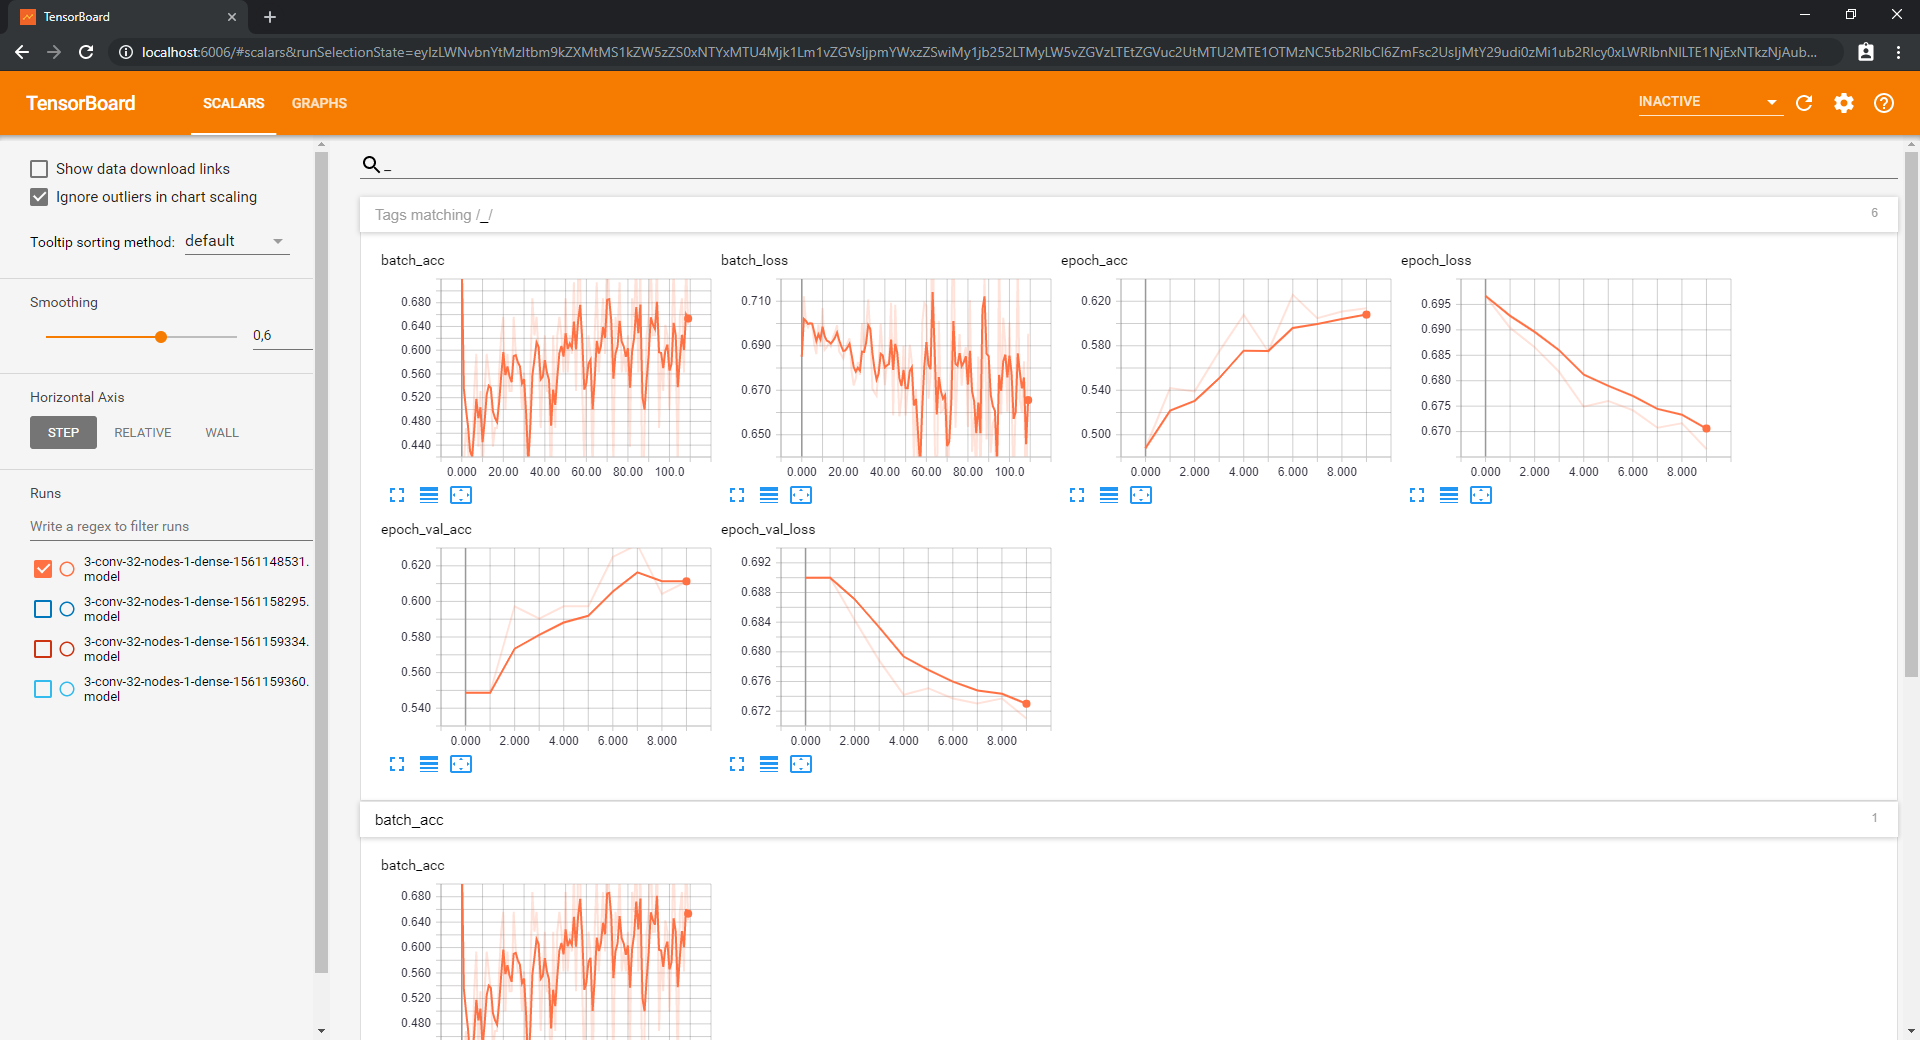
\includegraphics[scale=0.2]{tensorboard.png}
  \caption{Interfaccia iniziale di Tensorboard}
\end{figure}

Quindi questo strumento risulta molto utile per effettuare un'analisi dettagliata su come vari modelli sono composti e soprattutto su come performano. Ad esempio già nella schermata principale si può notare l’andamento dei principali parametri, loss e accuracy, per epoch o per batch. Inoltre navigando nella sezione \texttt{graph} tensorflow fornisce una visualizzazione a grafo del modello, ovvero vengono visualizzati i vari layers della rete specificando le loro connessioni e le variazioni di shape dei dati che passano attraverso la struttura.

\begin{figure}[h]
  \centering
  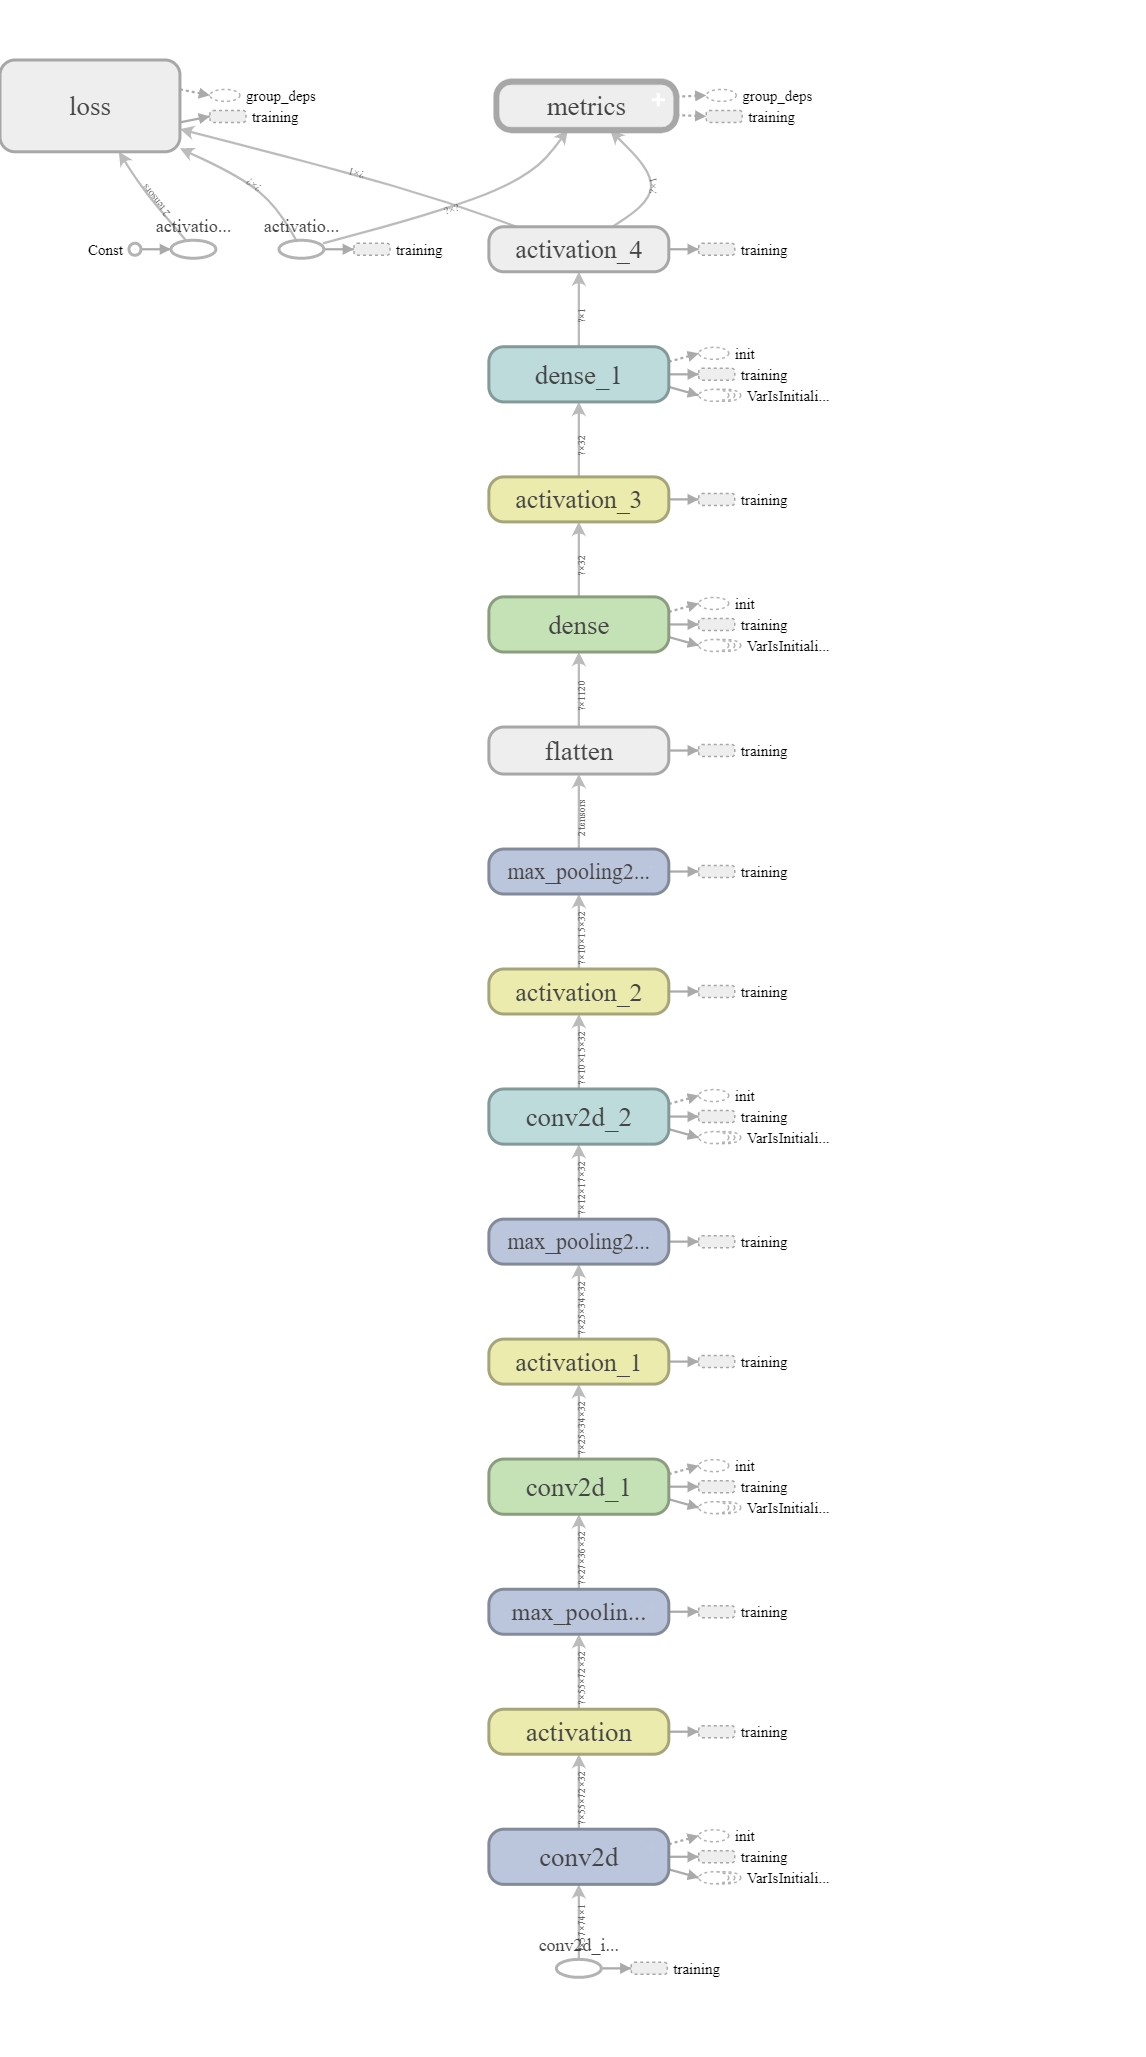
\includegraphics[scale=0.4]{grafo_rete.png}
  \caption{Esempio di grafo di rete prodotto da Tensorboard}
\end{figure}

Le potenzialità di Tensorboard non si limitano soltanto a delle visualizzazioni di grafici tuttavia già solo con questi strumenti si possono andare a comparare i principali parametri e i risultati di vari modelli in modo da capire quale modello si comporta meglio degli altri per il problema in esame.

Nell’elaborato si può abilitare il salvataggio dei log della fase di training, (utilizzati da Tensorboard per costruire i vari grafici) tramite il parametro \texttt{TENSORBOARD} presente nella sezione \texttt{NEURAL\_NETWORK\_TRAIN} del file di configurazione. In questo modo verranno salvati nella sottocartella \texttt{LOGS} di \texttt{MODELS} i logs associati ad ogni modello, poi in Tensorboard sarà possibile selezionare uno o più modelli per visualizzarne tutti i dati.
  
  \section{Predictions}
  La parte finale dell’elaborato consiste nell’utilizzare un modello già trainato per fargli produrre delle previsioni a fronte dell’inserimento di nuove immagini. Si sceglie quindi il modello dal quale si vogliono ottenere le previsioni, per far ciò basta copiare il file con estensione \texttt{.model}, corrispondente al modello scelto, nella cartella \texttt{PREDICTION}. Successivamente si inseriscono le immagini su cui si vuole avere un riscontro nella sottocartella di \texttt{PREDICTION}, \texttt{DATA\_TO\_PREDICT}. Infine si lancia lo script \texttt{predict.py}, che dopo un primo controllo sull’esistenza delle immagini e del modello nella cartella designata, invoca la funzione \texttt{make\_predictions} che al suo interno richiama la funzione \texttt{create\_data} di \texttt{preprocess.py}, in questo modo si fanno passare le nuove immagini attraverso tutte le diverse elaborazioni precedentemente descritte: filtri, threshold, Hough, segmentation e cropping. Grazie a questo passaggio si estraggono i segmenti di interesse dalle nuove immagini.

L’ultima operazione da effettuare prima di poter chiedere al modello di effettuare le previsioni è quella di resize dei nuovi segmenti. Infatti i segmenti prodotti da \texttt{create\_data} sotto generalmente di dimensione diversa, risulta quindi necessario ridimensionarli tutti alla stessa dimensione; tuttavia non li si può ridimensionare alla shape media come in precedenza, bisogna infatti ridimensionarli alla dimensione che il modello si aspetta di ricevere, in quanto il modello è stato addestrato per operare con immagini in input con quella particolare shape. La dimensione delle immagini in input richiesta dal modello è ottenibile accedendo all’attributo \texttt{input\_shape} dell’oggetto che rappresenta il modello stesso, successivamente si richiama la funzione \texttt{resize} di NumPy per ridimensionare i segmenti. 

A questo punto si può chiedere al modello di effettuare le previsioni, si richiama quindi la funzione \texttt{predict} sull’oggetto rappresentante il modello passandogli come parametro il vettore che contiene i segmenti ridimensionati. La funzione restituisce un array dove ogni elemento rappresenta il risultato della previsione per ogni immagine, se la previsione è 0 significa che la rete ha ritenuto il segmento come non problematico, mentre nel caso contrario ci sarà un 1 come previsione e quindi il segmento è stato reputato problematico. La funzione termina stampando sullo standard output il risultato della previsione associato al nome dell’immagine.

\begin{figure}[h]
  \centering
  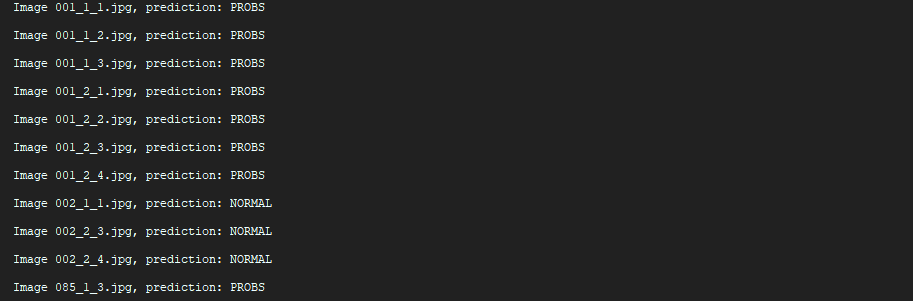
\includegraphics[width=1.0\textwidth]{predictions.png}
  \caption{Esempio di output ottenuto lanciando \texttt{predict.py}}
\end{figure}

  
  \setcounter{secnumdepth}{-1}
  \chapter{Conclusioni}
  Grazie a questo elaborato è stata approfondita la conoscenza dei vari metodi di elaborazione delle immagini, comprendendo la grande importanza della loro implementazione al fine di ottenere degli input ottimali per una rete neurale. Sono stati esplorati infatti diversi filtri in ambito biometrico, imparando ad utilizzare la libreria OpenCV per la loro strutturazione e applicazione.

Si sono compresi inoltre il funzionamento e la struttura delle Convolutional Neural Networks, branca del machine learning in continua evoluzione. In particolar modo sono state studiate le diverse funzioni dei layer che costituiscono un modello di una CNN, imparandone il funzionamento tipico in ambito di computer vision per un caso di classificazione binaria. La rete implementata è idealmente buona per un problema di questo tipo, ma i risultati ottenuti non sono stati considerati in quanto non si è potuta verificare l’effettiva validità dell’iridologia, in assenza di dati “reali” per il training della rete neurale. Ciononostante il progetto è aperto a futuri ampliamenti in tale ambito (e non solo), in quanto con i giusti dati si può effettivamente verificare la veridicità di questa teoria medica alternativa.

  
\end{document}
